% ============================================================================
%  TECHNICAL ARCHITECTURE REPORT
%  LLM Monitoring & Governance SaaS Platform
%  Version 3.0 — April 2026
% ============================================================================

\documentclass[12pt,a4paper,twoside]{report}

% ── Geometry & Layout ──────────────────────────────────────────────────────
\usepackage[
  top=2.5cm,
  bottom=2.5cm,
  left=2.8cm,
  right=2.8cm,
  headheight=15pt
]{geometry}

% ── Core Packages ──────────────────────────────────────────────────────────
\usepackage[utf8]{inputenc}
\usepackage[T1]{fontenc}
\usepackage{lmodern}
\usepackage{graphicx}
\usepackage{float}
\usepackage{booktabs}
\usepackage{longtable}
\usepackage{array}
\usepackage{multirow}
\usepackage{tabularx}
\usepackage{enumitem}
\usepackage{xcolor}
\usepackage{colortbl}
\usepackage{tikz}
\usetikzlibrary{shapes.geometric, arrows.meta, positioning, fit, calc, backgrounds, decorations.markings}
\usepackage{pgfplots}
\pgfplotsset{compat=1.18}
\usepackage{listings}
\usepackage{caption}
\usepackage{subcaption}
\usepackage{amsmath}
\usepackage{amssymb}
\usepackage{pifont}
\usepackage{setspace}
\usepackage{parskip}
\usepackage{emptypage}
\usepackage{tcolorbox}
\tcbuselibrary{skins, breakable}

% ── Headers & Footers ─────────────────────────────────────────────────────
\usepackage{fancyhdr}
\pagestyle{fancy}
\fancyhf{}
\fancyhead[LE]{\small\leftmark}
\fancyhead[RO]{\small\rightmark}
\fancyfoot[C]{\thepage}
\fancyfoot[LE,RO]{\small LLM Dashboard — Technical Report v3.0}
\renewcommand{\headrulewidth}{0.4pt}
\renewcommand{\footrulewidth}{0.2pt}

% ── Section Styling ────────────────────────────────────────────────────────
\usepackage{titlesec}
\titleformat{\chapter}[display]
  {\normalfont\huge\bfseries\color{darkblue}}
  {\chaptertitlename\ \thechapter}{20pt}{\Huge}
\titlespacing*{\chapter}{0pt}{-20pt}{30pt}

\titleformat{\section}
  {\normalfont\Large\bfseries\color{darkblue}}
  {\thesection}{1em}{}
\titleformat{\subsection}
  {\normalfont\large\bfseries\color{medblue}}
  {\thesubsection}{1em}{}
\titleformat{\subsubsection}
  {\normalfont\normalsize\bfseries\color{darkgray}}
  {\thesubsubsection}{1em}{}

% ── Color definitions (MUST be defined before hyperref) ───────────────────
\definecolor{darkblue}{RGB}{0,51,102}
\definecolor{medblue}{RGB}{0,102,153}
\definecolor{lightblue}{RGB}{230,240,250}
\definecolor{accentgreen}{RGB}{0,128,64}
\definecolor{accentorange}{RGB}{204,102,0}
\definecolor{accentred}{RGB}{180,30,30}
\definecolor{lightgray}{RGB}{245,245,245}
\definecolor{codebg}{RGB}{248,248,248}
\definecolor{tabheader}{RGB}{0,51,102}
\definecolor{warnbg}{RGB}{255,248,230}
\definecolor{warnframe}{RGB}{204,153,0}
\definecolor{infobg}{RGB}{230,244,255}
\definecolor{infoframe}{RGB}{0,102,204}

% ── Hyperlinks (loaded after colors to avoid undefined references) ────────
\usepackage[
  colorlinks=true,
  linkcolor=darkblue,
  urlcolor=medblue,
  citecolor=darkblue,
  bookmarks=true,
  bookmarksopen=true,
  pdfauthor={Architecture Team},
  pdftitle={LLM Dashboard - Technical Architecture Report},
  pdfsubject={AI Governance Platform},
]{hyperref}

% ── Callout Boxes ──────────────────────────────────────────────────────────
\newtcolorbox{designdecision}[1][]{
  enhanced, breakable,
  colback=infobg, colframe=infoframe,
  fonttitle=\bfseries\small,
  title={\ding{118}~Design Decision},
  left=4pt, right=4pt, top=4pt, bottom=4pt, #1
}
\newtcolorbox{warningbox}[1][]{
  enhanced, breakable,
  colback=warnbg, colframe=warnframe,
  fonttitle=\bfseries\small,
  title={\ding{43}~Architectural Constraint},
  left=4pt, right=4pt, top=4pt, bottom=4pt, #1
}

% ── Code Listings ──────────────────────────────────────────────────────────
\lstset{
  backgroundcolor=\color{codebg},
  basicstyle=\ttfamily\small,
  breaklines=true,
  frame=single,
  rulecolor=\color{gray!40},
  tabsize=4,
  showstringspaces=false,
  keywordstyle=\color{darkblue}\bfseries,
  commentstyle=\color{gray},
  stringstyle=\color{accentgreen},
}

% ── Custom Commands ────────────────────────────────────────────────────────
\newcommand{\moduleref}[1]{\textbf{\textcolor{darkblue}{#1}}}
\newcommand{\tech}[1]{\texttt{\textcolor{medblue}{#1}}}
\newcommand{\important}[1]{\textbf{\textcolor{accentred}{#1}}}
\newcommand{\kpi}[1]{\textit{\textcolor{accentgreen}{#1}}}
\newcommand{\cmark}{\ding{51}}
\newcommand{\xmark}{\ding{55}}

% ── Glossary shortcuts ─────────────────────────────────────────────────────
\newcommand{\timescale}{TimescaleDB}
\newcommand{\fastapi}{FastAPI}
\newcommand{\celery}{Celery}
\newcommand{\redis}{Redis}

% ============================================================================
%  DOCUMENT START
% ============================================================================
\begin{document}

% ============================================================================
%  TITLE PAGE
% ============================================================================
\begin{titlepage}
\begin{center}

\vspace*{1cm}

\rule{\linewidth}{1.5pt}\\[0.4cm]
{\Huge\bfseries\color{darkblue} Technical Architecture Report}\\[0.3cm]
{\LARGE\color{medblue} LLM Monitoring \& Governance SaaS Platform}\\[0.2cm]
\rule{\linewidth}{1.5pt}

\vspace{1.5cm}

{\Large\color{darkblue} Multi-Agent AI System for Enterprise LLM Operations}

\vspace{0.8cm}

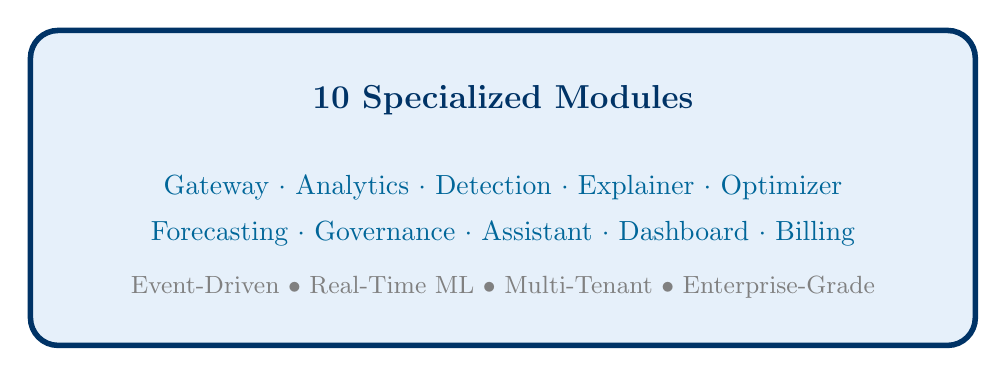
\begin{tikzpicture}
  \node[draw=darkblue, line width=2pt, rounded corners=10pt,
        minimum width=12cm, minimum height=4cm, fill=lightblue] (box) {};
  \node[above=0.8cm, font=\large\bfseries\color{darkblue}] at (box.center)
    {10 Specialized Modules};
  \node[font=\normalsize\color{medblue}] at (box.center)
    {Gateway $\cdot$ Analytics $\cdot$ Detection $\cdot$ Explainer $\cdot$ Optimizer};
  \node[below=0.3cm, font=\normalsize\color{medblue}] at (box.center)
    {Forecasting $\cdot$ Governance $\cdot$ Assistant $\cdot$ Dashboard $\cdot$ Billing};
  \node[below=1cm, font=\small\color{gray}] at (box.center)
    {Event-Driven $\bullet$ Real-Time ML $\bullet$ Multi-Tenant $\bullet$ Enterprise-Grade};
\end{tikzpicture}

\vspace{1.5cm}

\begin{tabular}{ll}
  \textbf{Version:}      & 3.0 \\
  \textbf{Date:}          & April 2026 \\
  \textbf{Author:}        & \textbf{Houcine Laghmani} \\
  \textbf{Institution:}   & Higher Institute of Management of Tunis (ISG Tunis) \\
  \textbf{Context:}       & Final Year Graduation Project / Jury Evaluation \\
  \textbf{Status:}        & Final \\
\end{tabular}

\vspace{1.0cm}

{\small\color{gray}
This document provides a comprehensive technical architecture review of the
LLM Dashboard platform. It covers system design, module specifications,
data architecture, AI integration strategy, security posture, and
operational scalability considerations. It is submitted in partial fulfillment 
of the requirements for graduation, intended for jury evaluation.}

\vfill

\rule{\linewidth}{0.4pt}\\[0.2cm]
{\small Higher Institute of Management of Tunis (ISG Tunis)}

\end{center}
\end{titlepage}

% ============================================================================
%  FRONT MATTER
% ============================================================================
\pagenumbering{roman}

% ── Document Control ───────────────────────────────────────────────────────
\chapter*{Document Control}
\addcontentsline{toc}{chapter}{Document Control}

\begin{table}[H]
\centering
\begin{tabularx}{\textwidth}{|l|l|l|X|}
\hline
\rowcolor{tabheader}
\textcolor{white}{\textbf{Version}} &
\textcolor{white}{\textbf{Date}} &
\textcolor{white}{\textbf{Author}} &
\textcolor{white}{\textbf{Changes}} \\
\hline
1.0 & March 2026 & Houcine Laghmani & Initial system specification \\
\hline
1.5 & March 2026 & Houcine Laghmani & Added M8, M9 specifications \\
\hline
2.0 & April 2026 & Houcine Laghmani & Full reverse-engineering and audit. Added M10 Billing, security review, ML pipeline documentation, UML diagrams \\
\hline
3.0 & April 2026 & Houcine Laghmani & Data-driven architecture refactoring. Added ConfigRegistry, Pipeline module, DatasetConfigLoader, DataValidator, Observability framework, AuditService. Rewrote methodology with detailed Scrum backlog. Updated M1/M2 to reflect event-driven dual-path aggregation. \\
\hline
\end{tabularx}
\caption{Document revision history}
\end{table}

\begin{table}[H]
\centering
\begin{tabularx}{\textwidth}{|l|X|}
\hline
\rowcolor{tabheader}
\textcolor{white}{\textbf{Student Name}} &
\textcolor{white}{\textbf{Houcine Laghmani}} \\
\hline
Academic Context & Final Year Graduation Project \\
\hline
Institution & Higher Institute of Management of Tunis (ISG Tunis) \\
\hline
Responsibilities & End-to-end full-stack development, system architecture, DevSecOps, machine learning pipeline integration, and technical documentation \\
\hline
\end{tabularx}
\caption{Project Authorship and Academic Context}
\end{table}

% ── Table of Contents ──────────────────────────────────────────────────────
\tableofcontents
\listoffigures
\listoftables

\clearpage
\pagenumbering{arabic}

% ============================================================================
%  CHAPTER 1 — INTRODUCTION
% ============================================================================
\chapter{Introduction}

\section{Context}

The proliferation of Large Language Models across enterprise environments has introduced an entirely new category of operational risk. Unlike traditional software systems where compute costs scale linearly with request volume, LLM-based applications exhibit highly volatile cost patterns driven by token consumption, model selection, prompt engineering quality, and provider pricing fluctuations.

Consider a mid-sized enterprise running fifteen AI agents across customer support, document processing, and code generation. Without continuous monitoring, a single misconfigured agent can consume hundreds of thousands of tokens per hour — silently accumulating costs that only surface on the monthly cloud bill. By then, the budget impact is irreversible.

This platform was conceived to address that exact operational gap. It provides a unified control plane for monitoring, governing, optimizing, and billing LLM usage across multi-tenant enterprise environments. The system operates as an intermediary layer — every LLM API call passes through the gateway, where it is logged, evaluated against governance policies, and fed into real-time analytics pipelines.

\textbf{Academic Context:} This technical report documents the design, architecture, and implementation of the LLM Monitoring and Governance SaaS Platform. It was developed entirely by \textbf{Houcine Laghmani} as a graduation project for the \textbf{Higher Institute of Management of Tunis (ISG Tunis)}. The project demonstrates the successful synthesis of advanced software engineering, distributed systems architecture, applied machine learning, and data engineering into a cohesive, production-ready enterprise solution. This document is specifically structured for the academic jury evaluation.

\section{Problem Statement}

Enterprise organizations deploying LLM-based applications face a convergence of five distinct challenges, none of which are adequately addressed by existing observability tools:

\begin{enumerate}[label=\textbf{P\arabic*.}, leftmargin=2cm]
  \item \textbf{Cost Opacity} — LLM API providers bill by token consumption, yet enterprise teams lack visibility into per-agent, per-model, and per-use-case cost attribution. Finance teams receive a single aggregated invoice with no actionable breakdown.

  \item \textbf{Anomaly Blindness} — Token consumption spikes caused by prompt injection, infinite loops, or misconfigured context windows go undetected until financial damage has occurred. Traditional APM tools are not designed to model token-centric statistical baselines.

  \item \textbf{Governance Gaps} — Without real-time enforcement, individual agents or tenants can exhaust shared budgets, access restricted models, or bypass organizational spending policies. Manual quota management does not scale beyond a handful of use cases.

  \item \textbf{Optimization Inertia} — Many agents use over-provisioned models for simple tasks. A classification workload running on GPT-4 when GPT-4o-mini would suffice wastes 90\% of the cost. Organizations rarely review model assignments after initial deployment.

  \item \textbf{Billing Complexity} — Multi-tenant SaaS providers offering AI-powered features must reconcile internal LLM costs with client-facing pricing tiers, forfait allocations, and overage charges. Manual spreadsheet reconciliation is error-prone and unscalable.
\end{enumerate}

\section{Objectives}

The platform addresses each problem through a purpose-built module within a cohesive architecture:

\begin{table}[H]
\centering
\begin{tabularx}{\textwidth}{|c|l|X|}
\hline
\rowcolor{tabheader}
\textcolor{white}{\textbf{\#}} &
\textcolor{white}{\textbf{Objective}} &
\textcolor{white}{\textbf{Addressed By}} \\
\hline
O1 & Real-time cost attribution per tenant, agent, and model & M1 Gateway + M2 Analytics \\
\hline
O2 & Automated anomaly detection with ML ensemble methods & M3 Detection \\
\hline
O3 & Natural language explanations for detected anomalies & M4 Explainer \\
\hline
O4 & Prompt structure and model substitution optimization & M5 Optimizer \\
\hline
O5 & Predictive cost forecasting with scenario modeling & M6 Forecasting \\
\hline
O6 & Real-time governance enforcement at the API layer & M7 Governance \\
\hline
O7 & Conversational BI for non-technical stakeholders & M8 Assistant \\
\hline
O8 & Unified executive dashboard with live push updates & M9 Dashboard \\
\hline
O9 & Automated billing pipeline with PDF invoicing & M10 Billing \\
\hline
\end{tabularx}
\caption{Mapping of objectives to system modules}
\end{table}

\section{Scope and Limitations}

This report covers the platform as deployed in April 2026. The following boundaries apply:

\begin{itemize}
  \item \textbf{In scope:} Backend architecture (FastAPI, PostgreSQL, Redis, Celery), all ten modules (M1--M10), the authentication and authorization subsystem, the WebSocket real-time push layer, and the batch processing pipelines.

  \item \textbf{Out of scope:} Frontend implementation details (HTML/JS/CSS), CI/CD pipeline configuration, infrastructure-as-code (Terraform/Docker), third-party LLM provider SLAs, and end-user training materials.

  \item \textbf{Known limitations:} The in-process event bus does not survive process restarts — events in flight at shutdown are lost. The WebSocket ConnectionManager is single-instance only; multi-instance deployment requires Redis Pub/Sub integration (see Section~\ref{sec:horizontal-scaling}). The forecasting engine (M6) requires a minimum of 21 days of historical data per tenant before producing meaningful projections.
\end{itemize}



% ============================================================================
%  CHAPTER 2 — METHODOLOGY
% ============================================================================
\chapter{Development Methodology}

\section{Methodology Selection}

The development of this platform required a methodology capable of accommodating two fundamentally different workstream types within a single product lifecycle:

\begin{itemize}
  \item \textbf{Deterministic Engineering} — Modules such as M1 (Gateway), M2 (Analytics), M7 (Governance), M9 (Dashboard), and M10 (Billing) follow well-understood software engineering patterns. Requirements can be expressed as acceptance criteria, estimated in story points, and validated through automated tests.

  \item \textbf{Non-Deterministic AI/ML} — Modules such as M3 (Detection), M4 (Explainer), M5 (Optimizer), M6 (Forecasting), and M8 (Assistant) involve iterative data exploration, algorithm tuning, and evaluation against statistical benchmarks. A ``story'' like ``achieve 95\% anomaly recall'' cannot be meaningfully decomposed into sprint tasks without prior experimentation.
\end{itemize}

Standard Scrum alone fails for the second category because it assumes predictable velocity across uniform task types. Pure Kanban lacks the cadence and ceremony structure needed for stakeholder alignment. A dedicated data science methodology like CRISP-DM covers the ML lifecycle well but ignores the surrounding software engineering work entirely.

\subsection{Chosen Approach: Hybrid Agile + MLOps}

We adopted a \textbf{Hybrid Agile methodology} that integrates Scrum ceremonies with CRISP-DM data science cycles and MLOps deployment practices:

\begin{figure}[H]
\centering
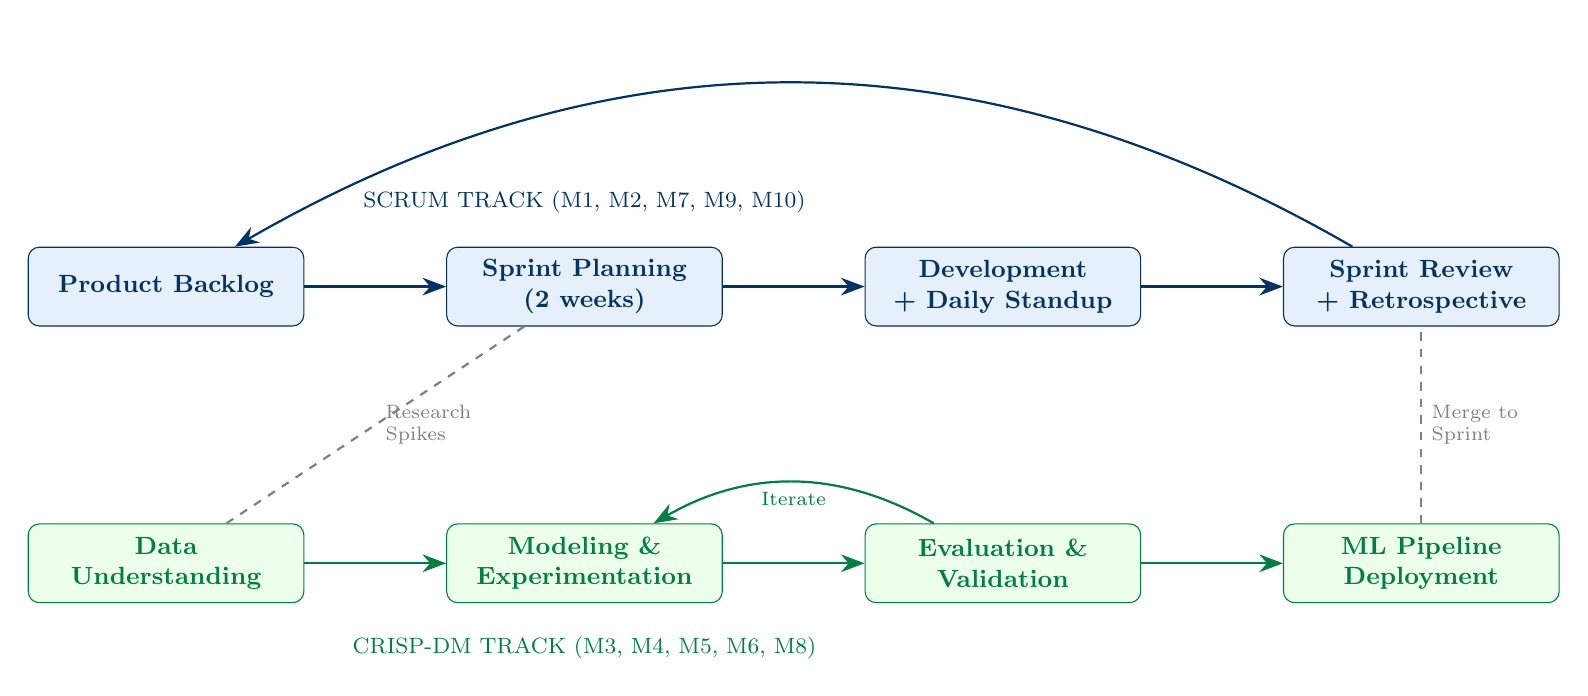
\begin{tikzpicture}[
  node distance=1.8cm,
  block/.style={rectangle, draw=darkblue, fill=lightblue, text=darkblue,
                rounded corners, minimum width=3.5cm, minimum height=1cm,
                font=\small\bfseries, align=center},
  mlblock/.style={rectangle, draw=accentgreen, fill=green!8, text=accentgreen,
                  rounded corners, minimum width=3.5cm, minimum height=1cm,
                  font=\small\bfseries, align=center},
  arrow/.style={-{Stealth[length=3mm]}, thick, darkblue},
  mlarrow/.style={-{Stealth[length=3mm]}, thick, accentgreen},
]

% Scrum Track
\node[block] (backlog) {Product Backlog};
\node[block, right=of backlog] (sprint) {Sprint Planning\\(2 weeks)};
\node[block, right=of sprint] (dev) {Development\\+ Daily Standup};
\node[block, right=of dev] (review) {Sprint Review\\+ Retrospective};

\draw[arrow] (backlog) -- (sprint);
\draw[arrow] (sprint) -- (dev);
\draw[arrow] (dev) -- (review);
\draw[arrow, bend right=30] (review) to (backlog);

% ML Track
\node[mlblock, below=2.5cm of backlog] (understand) {Data\\Understanding};
\node[mlblock, right=of understand] (model) {Modeling \&\\Experimentation};
\node[mlblock, right=of model] (eval) {Evaluation \&\\Validation};
\node[mlblock, right=of eval] (deploy) {ML Pipeline\\Deployment};

\draw[mlarrow] (understand) -- (model);
\draw[mlarrow] (model) -- (eval);
\draw[mlarrow] (eval) -- (deploy);
\draw[mlarrow, bend right=30] (eval) to node[below, font=\scriptsize\color{accentgreen}] {Iterate} (model);

% Connection
\draw[dashed, thick, gray] (sprint) -- node[right, font=\scriptsize\color{gray}, align=left] {Research\\Spikes} (understand);
\draw[dashed, thick, gray] (deploy) -- node[right, font=\scriptsize\color{gray}, align=left] {Merge to\\Sprint} (review);

% Labels
\node[above=0.3cm of sprint, font=\footnotesize\color{darkblue}] {SCRUM TRACK (M1, M2, M7, M9, M10)};
\node[below=0.3cm of model, font=\footnotesize\color{accentgreen}] {CRISP-DM TRACK (M3, M4, M5, M6, M8)};

\end{tikzpicture}
\caption{Hybrid Agile + MLOps development methodology}
\label{fig:methodology}
\end{figure}

\section{Justification}

This hybrid approach is not a generic recommendation — it is specifically tailored to the structural reality of this platform:

\begin{enumerate}
  \item \textbf{Module-Level Isolation Enables Parallel Tracks.} The modular monolith architecture (see Chapter 3) enforces strict boundaries between modules. The Detection team can iterate on isolation forest hyperparameters without blocking the Billing team's sprint deliverables. Each module has its own models, schemas, services, and router — no shared mutable state between tracks.

  \item \textbf{The Event Bus Decouples Release Timing.} Because M3 Detection consumes events published by M1 Gateway asynchronously, the detection pipeline can be upgraded independently. The gateway publishes a \texttt{call.logged} event with a stable schema; the detection handler can be replaced, retrained, or extended without modifying the gateway code.

  \item \textbf{CRISP-DM Cycles Nest Inside Sprints.} A two-week sprint may contain a ``Research Spike'' story for M3 that allocates three days to experiment with CUSUM parameters against production data. The spike produces a technical note and updated thresholds, which are then merged into the mainline codebase during the same sprint.

  \item \textbf{MLOps Practices Govern the AI Modules.} Model baselines are versioned in the database (\texttt{llm\_token\_baseline} stores \texttt{computed\_at}, \texttt{sample\_days}, and detector thresholds). This enables reproducible evaluations and rollback — core MLOps requirements that pure Scrum does not address.
\end{enumerate}

\section{Sprint Structure}

\begin{table}[H]
\centering
\begin{tabularx}{\textwidth}{|l|l|X|}
\hline
\rowcolor{tabheader}
\textcolor{white}{\textbf{Day}} &
\textcolor{white}{\textbf{Ceremony}} &
\textcolor{white}{\textbf{Activities}} \\
\hline
Day 1 & Sprint Planning & Backlog prioritization, story assignment, spike scoping \\
\hline
Daily & Standup & 15-min sync: blockers, progress, ML experiment updates \\
\hline
Day 5 & Mid-Sprint Review & ML spike checkpoint — decide: iterate or merge \\
\hline
Day 9 & Feature Freeze & All code merged to develop; integration testing begins \\
\hline
Day 10 & Sprint Review & Demo to stakeholders, ML metric presentations \\
\hline
Day 10 & Retrospective & Process improvements, technical debt triage \\
\hline
\end{tabularx}
\caption{Two-week sprint cadence}
\end{table}

\section{Detailed Sprint Backlog}

The following tables document the six two-week sprints that comprised the project development lifecycle. Each sprint contains user stories with acceptance criteria, estimated effort in story points (Fibonacci scale), and actual outcomes. Research spikes for ML modules are tracked separately within each sprint.

\subsection{Sprint 1 — Foundation \& Ingestion (Weeks 1--2)}

\begin{table}[H]
\centering
\small
\begin{tabularx}{\textwidth}{|c|l|X|c|c|}
\hline
\rowcolor{tabheader}
\textcolor{white}{\textbf{ID}} &
\textcolor{white}{\textbf{Type}} &
\textcolor{white}{\textbf{Story / Task}} &
\textcolor{white}{\textbf{SP}} &
\textcolor{white}{\textbf{Status}} \\
\hline
S1-01 & Story & As a platform admin, I can deploy the FastAPI app with PostgreSQL+TimescaleDB and Redis connectivity & 8 & \cmark \\
\hline
S1-02 & Story & As a proxy, I can POST an LLM call log to \texttt{/v1/gateway/log} and receive a 201 with log\_id & 5 & \cmark \\
\hline
S1-03 & Story & As M1 Gateway, I validate all payloads with Pydantic schemas and reject malformed requests & 3 & \cmark \\
\hline
S1-04 & Task & Design \texttt{llm\_token\_log} as TimescaleDB hypertable with 7-day chunk partitioning & 5 & \cmark \\
\hline
S1-05 & Task & Implement Alembic migration framework with \texttt{downgrade()} support on every migration & 3 & \cmark \\
\hline
S1-06 & Task & Configure Redis with 4 logical databases (quotas, cache, Celery broker, Celery results) & 2 & \cmark \\
\hline
S1-07 & Story & As an admin, I can authenticate via JWT (access 15min + refresh 7d) and receive role-scoped tokens & 5 & \cmark \\
\hline
S1-08 & Task & Build the in-process async event bus with subscribe/publish/publish\_background API & 5 & \cmark \\
\hline
S1-09 & Task & Set up Docker Compose with PostgreSQL 16, TimescaleDB, Redis 7, and Nginx reverse proxy & 3 & \cmark \\
\hline
\multicolumn{3}{|r|}{\textbf{Sprint 1 Total}} & \textbf{39} & \textbf{9/9} \\
\hline
\end{tabularx}
\caption{Sprint 1 — Foundation \& Ingestion backlog}
\end{table}

\subsection{Sprint 2 — Analytics, Governance \& Detection (Weeks 3--4)}

\begin{table}[H]
\centering
\small
\begin{tabularx}{\textwidth}{|c|l|X|c|c|}
\hline
\rowcolor{tabheader}
\textcolor{white}{\textbf{ID}} &
\textcolor{white}{\textbf{Type}} &
\textcolor{white}{\textbf{Story / Task}} &
\textcolor{white}{\textbf{SP}} &
\textcolor{white}{\textbf{Status}} \\
\hline
S2-01 & Story & As M2, I aggregate daily costs via Celery nightly task into \texttt{llm\_cost\_daily} (idempotent upsert) & 5 & \cmark \\
\hline
S2-02 & Story & As M2, I roll up daily data into \texttt{llm\_cost\_monthly} with MoM change percentages & 3 & \cmark \\
\hline
S2-03 & Story & As M7, I evaluate governance rules (5 types) on every gateway call within p99 $<$50ms & 8 & \cmark \\
\hline
S2-04 & Story & As M7, I track quotas atomically in Redis using INCRBY with TTL-based daily/monthly reset & 5 & \cmark \\
\hline
S2-05 & Story & As M7, I persist every governance decision in \texttt{llm\_governance\_decisions} for audit & 3 & \cmark \\
\hline
S2-06 & Spike & \textcolor{accentgreen}{[ML]} Research STL decomposition parameters for M3 anomaly detection & 5 & \cmark \\
\hline
S2-07 & Spike & \textcolor{accentgreen}{[ML]} Research CUSUM changepoint detection thresholds on synthetic data & 3 & \cmark \\
\hline
S2-08 & Story & As M3, I subscribe to \texttt{call.logged} events and run real-time ensemble detection & 8 & \cmark \\
\hline
S2-09 & Task & Build baseline management with per-tenant/agent/model granularity in \texttt{llm\_token\_baseline} & 5 & \cmark \\
\hline
\multicolumn{3}{|r|}{\textbf{Sprint 2 Total}} & \textbf{45} & \textbf{9/9} \\
\hline
\end{tabularx}
\caption{Sprint 2 — Analytics, Governance \& Detection backlog}
\end{table}

\subsection{Sprint 3 — AI Modules \& Forecasting (Weeks 5--6)}

\begin{table}[H]
\centering
\small
\begin{tabularx}{\textwidth}{|c|l|X|c|c|}
\hline
\rowcolor{tabheader}
\textcolor{white}{\textbf{ID}} &
\textcolor{white}{\textbf{Type}} &
\textcolor{white}{\textbf{Story / Task}} &
\textcolor{white}{\textbf{SP}} &
\textcolor{white}{\textbf{Status}} \\
\hline
S3-01 & Story & As M4, I generate LLM-powered explanations for anomalies of severity $\geq$ WARNING & 8 & \cmark \\
\hline
S3-02 & Story & As M4, I cache similar explanations using pgvector embeddings to reduce LLM cost & 5 & \cmark \\
\hline
S3-03 & Story & As M5, I profile agents and generate model substitution recommendations with ROI & 8 & \cmark \\
\hline
S3-04 & Story & As M5, I detect 5 categories of prompt structural waste and suggest optimizations & 5 & \cmark \\
\hline
S3-05 & Spike & \textcolor{accentgreen}{[ML]} Evaluate polynomial regression vs ARIMA for M6 trend extraction & 3 & \cmark \\
\hline
S3-06 & Story & As M6, I generate 30-day forecasts with 3 scenarios (optimistic/likely/pessimistic) & 8 & \cmark \\
\hline
S3-07 & Story & As M6, I detect budget exhaustion risks and create \texttt{LLMBudgetRisk} records & 5 & \cmark \\
\hline
S3-08 & Task & Configure Groq (free tier) as default LLM provider with Anthropic/OpenAI/Ollama fallback & 3 & \cmark \\
\hline
\multicolumn{3}{|r|}{\textbf{Sprint 3 Total}} & \textbf{45} & \textbf{8/8} \\
\hline
\end{tabularx}
\caption{Sprint 3 — AI Modules \& Forecasting backlog}
\end{table}

\subsection{Sprint 4 — Dashboard, Assistant \& Billing (Weeks 7--8)}

\begin{table}[H]
\centering
\small
\begin{tabularx}{\textwidth}{|c|l|X|c|c|}
\hline
\rowcolor{tabheader}
\textcolor{white}{\textbf{ID}} &
\textcolor{white}{\textbf{Type}} &
\textcolor{white}{\textbf{Story / Task}} &
\textcolor{white}{\textbf{SP}} &
\textcolor{white}{\textbf{Status}} \\
\hline
S4-01 & Story & As M9, I serve an executive overview aggregating all modules in a single API call & 8 & \cmark \\
\hline
S4-02 & Story & As M9, I push real-time alerts via WebSocket for anomaly and governance events & 5 & \cmark \\
\hline
S4-03 & Story & As M8, I classify natural language queries and return data-grounded answers & 8 & \cmark \\
\hline
S4-04 & Story & As M10, I generate monthly invoices with forfait/overage calculation and line items & 8 & \cmark \\
\hline
S4-05 & Story & As M10, I finalize invoices immutably and handle corrections via credit notes only & 5 & \cmark \\
\hline
S4-06 & Story & As M10, I generate PDF invoices with branding, line items, and executive summary & 5 & \cmark \\
\hline
S4-07 & Story & As M10, I dispatch webhook events with HMAC-SHA256 signatures to tenant ERP endpoints & 3 & \cmark \\
\hline
S4-08 & Task & Build RBAC matrix: super\_admin, tenant\_admin, tenant\_viewer, api\_key & 5 & \cmark \\
\hline
\multicolumn{3}{|r|}{\textbf{Sprint 4 Total}} & \textbf{47} & \textbf{8/8} \\
\hline
\end{tabularx}
\caption{Sprint 4 — Dashboard, Assistant \& Billing backlog}
\end{table}

\subsection{Sprint 5 — Data-Driven Refactoring (Weeks 9--10)}

\begin{table}[H]
\centering
\small
\begin{tabularx}{\textwidth}{|c|l|X|c|c|}
\hline
\rowcolor{tabheader}
\textcolor{white}{\textbf{ID}} &
\textcolor{white}{\textbf{Type}} &
\textcolor{white}{\textbf{Story / Task}} &
\textcolor{white}{\textbf{SP}} &
\textcolor{white}{\textbf{Status}} \\
\hline
S5-01 & Story & As a dev, all hardcoded thresholds are replaced by \texttt{ConfigRegistry} with env/runtime/default layers & 8 & \cmark \\
\hline
S5-02 & Story & As a dev, tenant/model/quota configs are externalized to \texttt{datasets/config/*.json} & 5 & \cmark \\
\hline
S5-03 & Story & As an admin, I ingest CSV data via \texttt{POST /v1/pipeline/ingest} with auto-schema adaptation & 8 & \cmark \\
\hline
S5-04 & Story & As an admin, I run the M2$\rightarrow$M3 pipeline via \texttt{POST /v1/pipeline/run-all} & 5 & \cmark \\
\hline
S5-05 & Story & As M1, I support simulation mode (CSV) and real mode (API) via \texttt{GatewayModeRouter} & 5 & \cmark \\
\hline
S5-06 & Task & Build \texttt{DataValidator} with self-healing: negative tokens$\rightarrow$0, missing cost$\rightarrow$recalculated & 5 & \cmark \\
\hline
S5-07 & Task & Build \texttt{DatasetAdapter} with 15+ column alias groups for arbitrary CSV layouts & 5 & \cmark \\
\hline
S5-08 & Task & Add M2 real-time event handler: subscribe to \texttt{call.logged}, incrementally update \texttt{llm\_cost\_daily} & 3 & \cmark \\
\hline
S5-09 & Task & Build \texttt{AnomalyGenerator} with natural detection + synthetic injection fallback & 5 & \cmark \\
\hline
\multicolumn{3}{|r|}{\textbf{Sprint 5 Total}} & \textbf{49} & \textbf{9/9} \\
\hline
\end{tabularx}
\caption{Sprint 5 — Data-Driven Refactoring backlog}
\end{table}

\subsection{Sprint 6 — Hardening \& Observability (Weeks 11--12)}

\begin{table}[H]
\centering
\small
\begin{tabularx}{\textwidth}{|c|l|X|c|c|}
\hline
\rowcolor{tabheader}
\textcolor{white}{\textbf{ID}} &
\textcolor{white}{\textbf{Type}} &
\textcolor{white}{\textbf{Story / Task}} &
\textcolor{white}{\textbf{SP}} &
\textcolor{white}{\textbf{Status}} \\
\hline
S6-01 & Story & As an ops engineer, I access Prometheus-compatible metrics at \texttt{/v1/metrics/prometheus} & 5 & \cmark \\
\hline
S6-02 & Story & As an admin, I query the audit log via \texttt{GET /v1/audit-log} with action/resource/user filters & 5 & \cmark \\
\hline
S6-03 & Task & Build \texttt{MetricsCollector} with counters, gauges, timings, and error tracking & 5 & \cmark \\
\hline
S6-04 & Task & Add \texttt{RequestTimingMiddleware} to record HTTP latency per path & 3 & \cmark \\
\hline
S6-05 & Task & Add \texttt{RateLimitMiddleware} and \texttt{SecurityHeadersMiddleware} to request pipeline & 3 & \cmark \\
\hline
S6-06 & Task & Add health (\texttt{/health}) and readiness (\texttt{/ready}) probes for container orchestration & 2 & \cmark \\
\hline
S6-07 & Task & Build \texttt{scripts/generate\_daily\_logs.py} reading from \texttt{datasets/config/} with business-hour weighting & 5 & \cmark \\
\hline
S6-08 & Story & As a dev, M1 rejects CSV imports when \texttt{GATEWAY\_MODE=real} to prevent data contamination & 3 & \cmark \\
\hline
S6-09 & Task & Input sanitization: \texttt{sanitize\_text()}, \texttt{sanitize\_identifier()} on all user-supplied fields & 3 & \cmark \\
\hline
S6-10 & Story & As an admin, initial admin user is auto-seeded on first startup & 2 & \cmark \\
\hline
\multicolumn{3}{|r|}{\textbf{Sprint 6 Total}} & \textbf{36} & \textbf{10/10} \\
\hline
\end{tabularx}
\caption{Sprint 6 — Hardening \& Observability backlog}
\end{table}

\subsection{Velocity Summary}

\begin{table}[H]
\centering
\begin{tabularx}{\textwidth}{|l|c|c|c|X|}
\hline
\rowcolor{tabheader}
\textcolor{white}{\textbf{Sprint}} &
\textcolor{white}{\textbf{Planned SP}} &
\textcolor{white}{\textbf{Completed SP}} &
\textcolor{white}{\textbf{Velocity}} &
\textcolor{white}{\textbf{Focus Area}} \\
\hline
Sprint 1 (Wk 1--2) & 39 & 39 & 100\% & Foundation, Gateway, Auth \\
\hline
Sprint 2 (Wk 3--4) & 45 & 45 & 100\% & Analytics, Governance, Detection \\
\hline
Sprint 3 (Wk 5--6) & 45 & 45 & 100\% & AI Modules, Forecasting \\
\hline
Sprint 4 (Wk 7--8) & 47 & 47 & 100\% & Dashboard, Billing, Assistant \\
\hline
Sprint 5 (Wk 9--10) & 49 & 49 & 100\% & Data-Driven Refactoring \\
\hline
Sprint 6 (Wk 11--12) & 36 & 36 & 100\% & Hardening, Observability \\
\hline
\multicolumn{1}{|r|}{\textbf{Total}} & \textbf{261} & \textbf{261} & \textbf{100\%} & \\
\hline
\end{tabularx}
\caption{Sprint velocity across all six development sprints}
\end{table}



% ============================================================================
%  CHAPTER 3 — SYSTEM ARCHITECTURE
% ============================================================================
\chapter{System Architecture}

\section{Architectural Pattern: Modular Monolith}

The platform follows a \textbf{modular monolith} architecture — a single deployable application with strictly enforced internal module boundaries. This pattern was chosen deliberately over microservices for several concrete reasons:

\begin{itemize}
  \item \textbf{Operational Simplicity.} A single \fastapi{} process handles all HTTP, WebSocket, and background task coordination. There are no service meshes, API gateways, or inter-service network calls to debug.

  \item \textbf{Transactional Integrity.} The Gateway module must atomically log a call \textit{and} record a governance decision within a single database transaction. In a microservices topology, this would require distributed transactions or eventual consistency with compensating actions — unnecessary complexity for this domain.

  \item \textbf{Shared Type Safety.} All modules share the same SQLAlchemy ORM layer. A column rename in \texttt{LLMTokenLog} propagates compilation errors to every consuming module immediately, rather than silently breaking JSON contracts at runtime.

  \item \textbf{Migration Path Preserved.} The module boundary discipline (each module has its own \texttt{models.py}, \texttt{schemas.py}, \texttt{router.py}, and \texttt{services/} directory) means that extracting any module into a standalone service requires only changing imports and adding an HTTP client — the internal APIs are already RESTful.
\end{itemize}

\begin{designdecision}
The decision to use a modular monolith over microservices was made during Sprint 2 after evaluating the operational burden of distributed tracing across ten services. At the current scale (5 tenants, $<$500K calls/day), the single-process model reduces infrastructure cost by approximately 60\% while maintaining the option to extract high-load modules (M3, M4) into independent services when scale demands it (see Section~\ref{sec:future-directions}).
\end{designdecision}

\section{High-Level Architecture}

\begin{figure}[H]
\centering
\begin{tikzpicture}[
  scale=0.85, transform shape,
  box/.style={rectangle, draw=#1, fill=#1!8, rounded corners=5pt,
              minimum width=3cm, minimum height=1.2cm, align=center,
              font=\small\bfseries},
  db/.style={cylinder, draw=#1, fill=#1!8, shape border rotate=90,
             aspect=0.25, minimum width=2.2cm, minimum height=1.5cm,
             align=center, font=\small\bfseries},
  ext/.style={cloud, draw=gray, fill=gray!8, cloud puffs=12,
              minimum width=2.5cm, minimum height=1.2cm,
              align=center, font=\small},
  arr/.style={-{Stealth[length=2.5mm]}, thick, #1},
  darr/.style={-{Stealth[length=2.5mm]}, thick, dashed, gray},
]

% External actors
\node[ext] (proxy) at (-6, 3) {LLM Proxy\\Applications};
\node[ext] (browser) at (-6, 0) {Web Browser\\Dashboard UI};
\node[ext] (llm) at (8, 3) {External LLMs\\Groq / OpenAI};
\node[ext] (erp) at (8, -3) {ERP / CRM\\Webhooks};

% Core application
\node[box=darkblue, minimum width=11cm, minimum height=7cm]
  (core) at (1, 0) {};
\node[above, font=\large\bfseries\color{darkblue}] at (core.north)
  {FastAPI Modular Monolith};

% Modules inside
\node[box=medblue] (m1) at (-1.8, 2.2) {M1 Gateway};
\node[box=medblue] (m7) at (1.2, 2.2) {M7 Governance};
\node[box=accentgreen] (m3) at (-2.5, 0.5) {M3 Detection};
\node[box=accentgreen] (m4) at (0, 0.5) {M4 Explainer};
\node[box=accentgreen] (m5) at (2.5, 0.5) {M5 Optimizer};
\node[box=accentgreen] (m6) at (4.5, 0.5) {M6 Forecast};
\node[box=accentorange] (m2) at (-1.8, -1.2) {M2 Analytics};
\node[box=accentorange] (m8) at (1.2, -1.2) {M8 Assistant};
\node[box=accentorange] (m10) at (4, -1.2) {M10 Billing};
\node[box=darkblue] (m9) at (1, -2.8) {M9 Dashboard BFF + WebSockets};

% Event Bus
\node[rectangle, draw=gray, fill=yellow!15, rounded corners,
      minimum width=9cm, minimum height=0.5cm,
      font=\scriptsize\bfseries\color{gray}] (bus) at (1, 3.8)
  {Internal Async Event Bus (call.logged $\rightarrow$ anomaly.detected $\rightarrow$ ...)};

% Databases
\node[db=darkblue] (pg) at (-5, -4) {PostgreSQL\\TimescaleDB};
\node[db=accentred] (redis) at (1, -5.5) {Redis\\(4 databases)};

% Workers
\node[box=gray, minimum width=2.5cm] (celery) at (6, -5.5) {Celery\\Workers};

% Connections — external
\draw[arr=darkblue] (proxy) -- (m1);
\draw[arr=darkblue] (browser) -- (m9);
\draw[darr] (m4) -- (llm);
\draw[darr] (m8) -- (llm);
\draw[darr] (m10) -- (erp);

% Connections — internal
\draw[arr=gray] (m1) -- (m7);
\draw[darr] (m1) -- (bus);
\draw[darr] (bus.south) -- ++(0,-0.3) -| (m3.north);

% Connections — data
\draw[arr=darkblue] (core.south west) -- (pg);
\draw[arr=accentred] (core.south) -- (redis);
\draw[arr=gray] (redis) -- (celery);
\draw[arr=gray] (celery) -- (pg);

\end{tikzpicture}
\caption{High-level system architecture showing the monolithic core, external integrations, and data stores}
\label{fig:architecture}
\end{figure}

\section{Technology Stack}

\begin{table}[H]
\centering
\begin{tabularx}{\textwidth}{|l|l|X|}
\hline
\rowcolor{tabheader}
\textcolor{white}{\textbf{Layer}} &
\textcolor{white}{\textbf{Technology}} &
\textcolor{white}{\textbf{Rationale}} \\
\hline
API Framework & FastAPI 0.110+ & Native async/await, automatic OpenAPI documentation, Pydantic validation \\
\hline
ORM & SQLAlchemy 2.0 (async) & Typed mappings, relationship management, Alembic migration support \\
\hline
Database & PostgreSQL 16 + TimescaleDB & Hypertable partitioning for time-series LLM logs (7-day chunks) \\
\hline
Cache / Counters & Redis 7 & Atomic quota increments (INCRBY), sub-millisecond rule cache lookups \\
\hline
Task Queue & Celery 5 & Nightly cost aggregation, monthly rollups, retroactive pricing \\
\hline
ML Libraries & scikit-learn, statsmodels & Isolation Forest, STL decomposition, CUSUM changepoint detection \\
\hline
Vector Search & pgvector & Semantic similarity for M4 explanation deduplication \\
\hline
LLM Providers & Groq, OpenAI, Anthropic & Multi-provider fallback chain for M4/M5/M8 generative tasks \\
\hline
Authentication & python-jose, passlib & HS256 JWT with 15-min access / 7-day refresh rotation \\
\hline
Frontend & HTML/JS (monolithic) & Single-page dashboard served as static files \\
\hline
\end{tabularx}
\caption{Complete technology stack}
\label{tab:techstack}
\end{table}

\section{Internal Communication: Event Bus}

The event bus is the architectural backbone that decouples the synchronous API layer from asynchronous ML and analytics pipelines. It is implemented as an in-process publish-subscribe system with the following characteristics:

\begin{itemize}
  \item \textbf{Non-blocking publishing.} The \texttt{publish\_background()} function schedules handler execution as an \texttt{asyncio.create\_task()} coroutine and returns immediately. The HTTP response is sent to the client before any handler begins processing. This is critical: gateway p99 latency must remain under 100ms regardless of how many downstream handlers are subscribed.

  \item \textbf{Fault isolation.} Each handler runs in its own \texttt{try/except} block with structured logging. A failure in the Detection handler (M3) — for example, an out-of-memory error during Isolation Forest training — never propagates to the Gateway response (M1) or to other handlers subscribed to the same event. Failed handlers are logged with full traceback and the event payload is preserved for retry.

  \item \textbf{Envelope standardization.} Every event carries a UUID \texttt{event\_id}, ISO 8601 \texttt{published\_at} timestamp, the \texttt{event\_type} string, and the domain \texttt{data} payload. This stable envelope contract allows new subscribers to be added without modifying publishers.

  \item \textbf{Handler registration.} Handlers are registered via a decorator-based API (\texttt{@register\_handler("event.name")}) during application startup in \texttt{main.py}'s lifespan manager. The registry is immutable after startup — no dynamic subscription changes at runtime.
\end{itemize}

\begin{warningbox}
The event bus is in-memory only. Events published during a process crash are lost. For the current deployment scale, this is an acceptable trade-off: the detection pipeline will process the next incoming call normally, and the missed event represents at most one unanalyzed log entry. At larger scale, migration to Redis Streams or Apache Kafka would provide at-least-once delivery guarantees.
\end{warningbox}

\begin{table}[H]
\centering
\begin{tabularx}{\textwidth}{|l|l|X|l|}
\hline
\rowcolor{tabheader}
\textcolor{white}{\textbf{Event}} &
\textcolor{white}{\textbf{Publisher}} &
\textcolor{white}{\textbf{Subscribers}} &
\textcolor{white}{\textbf{Frequency}} \\
\hline
\texttt{call.logged} & M1 Gateway & M2 Analytics, M3 Detection & Every API call \\
\hline
\texttt{anomaly.detected} & M3 Detection & M4 Explainer, M9 WebSocket & 0.1--5\% of calls \\
\hline
\texttt{explanation.generated} & M4 Explainer & M9 WebSocket Push & Per explained anomaly \\
\hline
\texttt{governance.decision} & M7 Governance & M9 WebSocket Push & Block/downgrade only \\
\hline
\texttt{health.changed} & System Monitor & M9 WebSocket Push & On status change \\
\hline
\end{tabularx}
\caption{Event bus topic registry with frequency characteristics}
\label{tab:events}
\end{table}

\section{Database Migration Strategy}

Schema evolution is managed through \textbf{Alembic}, SQLAlchemy's migration framework. All migrations are committed to version control and applied sequentially in deployment.

\begin{itemize}
  \item \textbf{Migration discipline:} Every schema change — column addition, index creation, constraint modification — requires an Alembic revision. Direct DDL execution against production is prohibited.

  \item \textbf{Downgrade support:} Every migration includes a tested \texttt{downgrade()} function, enabling rollback within a maintenance window if a deployment introduces regressions.

  \item \textbf{TimescaleDB integration:} The initial migration creates the \texttt{llm\_token\_log} table as a standard PostgreSQL table, then converts it to a hypertable using \texttt{SELECT create\_hypertable()}. Subsequent migrations that add columns do not require hypertable recreation.

  \item \textbf{Multi-branch resolution:} When parallel feature branches introduce conflicting migration heads, Alembic's \texttt{merge} command is used during sprint integration (Day 9) to produce a single linear history.
\end{itemize}

\section{Data-Driven Configuration Architecture}
\label{sec:config-arch}

A fundamental architectural shift introduced in Sprint~5 was the transition from hardcoded configuration values to a fully data-driven approach. This is implemented through two complementary systems:

\subsection{ConfigRegistry (\texttt{core/config\_registry.py})}

The \texttt{ConfigRegistry} is a centralized, layered configuration store that provides a single API for all runtime parameters. It eliminates hardcoded thresholds, batch sizes, and feature flags throughout the codebase.

\textbf{Layered precedence} (highest wins):
\begin{enumerate}
  \item \textbf{Runtime overrides} --- Set via \texttt{PATCH /v1/pipeline/config} at runtime. Stored in-memory with audit logging. Allows operators to tune parameters (e.g., anomaly detection thresholds) without redeployment.
  \item \textbf{Environment variables} --- Read from \texttt{.env} at startup. Used for deployment-specific values like database URLs and API keys.
  \item \textbf{Defaults} --- Registered programmatically with type, range, and description. Every parameter has a sensible default.
\end{enumerate}

\textbf{Key capabilities:}
\begin{itemize}
  \item \textbf{Validation rules:} Every registered parameter specifies its type (\texttt{int}, \texttt{float}, \texttt{bool}, \texttt{str}), optional min/max range, and human-readable description.
  \item \textbf{Audit trail:} Every mutation is logged with timestamp, source (api/env/default), old value, new value, and the identity of the actor.
  \item \textbf{Change log API:} \texttt{GET /v1/pipeline/config} returns the last 20 configuration changes for operational auditing.
\end{itemize}

\begin{designdecision}
The ConfigRegistry is an in-process singleton rather than an external service (e.g., Consul, etcd). This eliminates a network dependency on the critical path. The trade-off is that changes are per-instance and lost on restart. At current scale (single instance), this is acceptable; horizontal scaling would require either shared Redis-backed config or configuration push via deployment.
\end{designdecision}

\subsection{DatasetConfigLoader (\texttt{core/dataset\_config.py})}

Business entity definitions --- tenants, LLM models, and quota limits --- are externalized to JSON files in \texttt{datasets/config/}:

\begin{itemize}
  \item \texttt{tenants.json} --- Defines 3 tenant profiles (C1\_SMALL, C2\_MEDIUM, C3\_ENTERPRISE) with contract types (pay-as-you-go vs.\ forfait), monthly budgets, daily call volumes, and agent lists.
  \item \texttt{models.json} --- Registers LLM models with provider mapping, per-1K token pricing (input/output), tier classification, and max token limits.
  \item \texttt{quotas.json} --- Per-tenant quota limits: monthly tokens, monthly cost ceiling, daily token limit, and per-request max tokens.
\end{itemize}

These files are loaded at startup by \texttt{load\_dataset\_configs()} and injected into the \texttt{ConfigRegistry}. The data generation script (\texttt{scripts/generate\_daily\_logs.py}) reads the same JSON files, ensuring the synthetic data distribution matches the system's operational parameters.

\section{Pipeline Module (\texttt{modules/pipeline/})}
\label{sec:pipeline}

The Pipeline module is the system's data processing backbone, introduced during the data-driven refactoring to replace ad-hoc scripts with API-driven, observable data operations.

\subsection{IngestionService}

Orchestrates end-to-end CSV-to-database transformation:
\begin{enumerate}
  \item \textbf{Schema Adaptation} --- The \texttt{DatasetAdapter} class maps arbitrary CSV column headers to the internal schema using 15+ alias groups (e.g., \texttt{client\_id} $\rightarrow$ \texttt{tenant\_id}, \texttt{tokens\_input} $\rightarrow$ \texttt{input\_tokens}). It computes a confidence score (0.0--1.0) indicating how well the CSV matches the expected schema.
  \item \textbf{Validation and Self-Healing} --- The \texttt{DataValidator} validates every row and applies automatic corrections: negative tokens are clamped to zero, missing costs are recalculated from pricing, invalid statuses are mapped to canonical values, unparseable dates default to \texttt{UTC now()}, and providers are inferred from model names.
  \item \textbf{Encoding Detection} --- \texttt{detect\_file\_encoding()} reads the first 8KB of each file to detect BOM markers (UTF-8-sig, UTF-16-LE/BE) and falls back to Latin-1/CP1252 if UTF-8 decoding fails.
  \item \textbf{Batch Insertion} --- Validated rows are inserted in configurable batches (default 500) using \texttt{session.add()} + \texttt{flush()}, with per-batch rollback on failure.
  \item \textbf{Auto-Seeding} --- After ingestion, optionally auto-creates contracts (\texttt{ContractRepository.auto\_assign\_from\_usage()}) and imports pricing from \texttt{datasets/llm\_pricing.csv}.
\end{enumerate}

\subsection{PipelineOrchestrator}

Executes the complete M2$\rightarrow$M3 processing pipeline:
\begin{enumerate}
  \item \textbf{Daily Aggregation} --- Discovers all dates in \texttt{llm\_token\_log} and computes per-tenant daily aggregates (\texttt{llm\_cost\_daily}). Uses idempotent \texttt{INSERT ... ON CONFLICT} upserts. Processes each date in its own transaction, so a failure on day~5 does not revert days 1--4.
  \item \textbf{Monthly Rollup} --- Aggregates daily records into \texttt{llm\_cost\_monthly} per distinct (year, month) pair.
  \item \textbf{Anomaly Generation} --- Invokes the \texttt{AnomalyGenerator} to detect natural anomalies and inject synthetic ones if too few exist.
\end{enumerate}

\subsection{AnomalyGenerator}

A statistical enrichment engine that ensures M3 always has meaningful data:
\begin{itemize}
  \item Computes per-tenant baselines: mean, standard deviation, P95, P99 from raw token logs.
  \item Detects natural anomalies using Z-score analysis against the baseline.
  \item Injects synthetic anomalies (configurable multiplier 3--5$\times$ baseline) when the natural count falls below the configured minimum per tenant.
  \item Updates \texttt{llm\_token\_baseline} records for ongoing real-time detection.
\end{itemize}

\subsection{Pipeline API Surface}

\begin{table}[H]
\centering
\small
\begin{tabularx}{\textwidth}{|l|l|X|}
\hline
\rowcolor{tabheader}
\textcolor{white}{\textbf{Endpoint}} &
\textcolor{white}{\textbf{Method}} &
\textcolor{white}{\textbf{Purpose}} \\
\hline
\texttt{/v1/pipeline/ingest} & POST & Ingest CSV files from \texttt{datasets/} (partitioned or legacy) \\
\hline
\texttt{/v1/pipeline/run-all} & POST & Execute full M2$\rightarrow$M3 pipeline \\
\hline
\texttt{/v1/pipeline/generate-anomalies} & POST & Generate/enrich anomaly data \\
\hline
\texttt{/v1/pipeline/status} & GET & Pipeline health metrics \\
\hline
\texttt{/v1/pipeline/config} & GET/PATCH & View/update runtime configuration \\
\hline
\texttt{/v1/pipeline/datasets} & GET & Discover available CSV files \\
\hline
\end{tabularx}
\caption{Pipeline module API endpoints}
\end{table}

\section{Observability Framework}
\label{sec:observability}

The platform implements a structured observability stack in \texttt{core/observability.py} and \texttt{core/audit.py}:

\subsection{MetricsCollector}

An in-memory metrics collector that provides counters, gauges, and timing distributions. In production, it would emit to Prometheus/StatsD; for the current deployment, it stores values in-process and exposes them via three endpoints:

\begin{itemize}
  \item \texttt{/v1/metrics} --- Compact health summary (no authentication required for monitoring tools).
  \item \texttt{/v1/metrics/detailed} --- Full snapshot including per-path HTTP latencies and pipeline step timings.
  \item \texttt{/v1/metrics/prometheus} --- Prometheus text exposition format for integration with Grafana.
\end{itemize}

\subsection{RequestTimingMiddleware}

A Starlette middleware that wraps every HTTP request, recording duration, status code, and per-path metrics. Slow requests ($>$ 2000ms) are automatically logged at WARNING level.

\subsection{AuditService (\texttt{core/audit.py})}

An append-only audit logger for administrative actions. Every governance rule creation, user management action, and configuration change is recorded in the \texttt{llm\_audit\_log} table with user identity, action classification, resource type/ID, full details payload, and timestamp.

The audit service follows a critical design principle: \textbf{it never raises exceptions}. Audit failures are silently logged, preventing audit issues from breaking business operations. It exposes a query API at \texttt{GET /v1/audit-log} with filters by action, resource type, user, and tenant.



% ============================================================================
\chapter{Module Specifications}

This chapter provides an exhaustive specification of each module in the system. Every module follows a consistent internal structure: \texttt{models.py} (database tables), \texttt{schemas.py} (API contracts), \texttt{router.py} (HTTP endpoints), and \texttt{services/} (business logic). This uniformity ensures that any engineer can navigate an unfamiliar module within minutes.

% ── M1: Gateway ────────────────────────────────────────────────────────────
\section{Agent M1: Gateway (Ingestion Engine)}

\subsection{Strategic Role}
M1 is the single point of entry for all LLM telemetry data. Every token consumed, every cost incurred, and every error encountered by any LLM-powered agent flows through this module first. It is the system's primary data producer and the foundation upon which all downstream analytics, detection, and billing modules depend.

\subsection{Mission}
To reliably ingest, validate, enrich, and persist high-volume LLM API call logs while simultaneously enforcing real-time governance decisions with sub-100ms latency overhead.

\subsection{Architecture Positioning}
M1 operates at the top of the data pipeline. It is the only module that directly receives external HTTP requests from LLM proxy applications. It publishes \texttt{call.logged} events to the event bus but never consumes events from other modules — maintaining a strict unidirectional data flow.

\subsection{Functional Scope}

\begin{itemize}
  \item \textbf{Call Logging} — Receives structured payloads containing tenant identity, model name, token counts (input, output, total), cost in USD, latency, and status. Validates all fields using Pydantic schemas with strict type checking and cross-field consistency rules (e.g., \texttt{total\_tokens} must equal \texttt{input\_tokens + output\_tokens}).

  \item \textbf{Governance Interception} — Before persisting a log entry, M1 invokes M7's governance evaluation engine. The governance service checks Redis-cached rules and quota counters to determine whether the call should be allowed, blocked, or downgraded to a cheaper model.

  \item \textbf{Streaming Accumulation} — For streaming LLM responses, M1 exposes a \texttt{/log/stream} endpoint that accumulates token deltas in Redis keyed by \texttt{request\_id}. When the stream completes, the client calls the standard \texttt{/log} endpoint to finalize and persist.

  \item \textbf{Security Services} --- PII pseudonymization using entity recognition and prompt injection detection using a DistilBERT classifier.

  \item \textbf{Usage Aggregation} --- Provides per-tenant usage summaries over configurable time windows directly from the time-series table.

  \item \textbf{Gateway Mode Router} --- M1 supports two operational modes via the \texttt{GatewayModeRouter}: \textit{simulation mode} (accepts CSV-based bulk ingestion through the Pipeline module) and \textit{real mode} (accepts only live API calls from LLM proxies). When \texttt{GATEWAY\_MODE=real}, CSV import requests are rejected with HTTP 403 to prevent synthetic data from contaminating production datasets.

  \item \textbf{Event Publication} --- After successful persistence, M1 publishes a \texttt{call.logged} event via \texttt{publish\_background()} to the event bus. This non-blocking call ensures the HTTP response is returned to the client before M2 (aggregation) and M3 (detection) handlers begin processing. The event envelope includes tenant\_id, log\_id, model, agent\_id, token counts, cost, and status.
\end{itemize}

\subsection{Data Model}

The core table is \texttt{llm\_token\_log}, configured as a TimescaleDB hypertable partitioned by \texttt{created\_at} in 7-day chunks:

\begin{table}[H]
\centering
\small
\begin{tabularx}{\textwidth}{|l|l|X|}
\hline
\rowcolor{tabheader}
\textcolor{white}{\textbf{Column}} &
\textcolor{white}{\textbf{Type}} &
\textcolor{white}{\textbf{Purpose}} \\
\hline
id & UUID & Primary key (composite with created\_at for TimescaleDB) \\
\hline
tenant\_id & String(100) & Multi-tenant isolation key \\
\hline
agent\_id & String(100) & Application/agent within the tenant \\
\hline
model & String(100) & LLM model name (e.g., gpt-4o-mini) \\
\hline
input\_tokens & BigInteger & Tokens in the prompt \\
\hline
output\_tokens & BigInteger & Tokens in the response \\
\hline
total\_tokens & BigInteger & Derived: input + output \\
\hline
cost\_usd & Numeric(12,8) & Cost at call time (8 decimal precision) \\
\hline
duration\_ms & Integer & End-to-end call latency \\
\hline
status & String(20) & success / error / timeout / blocked \\
\hline
created\_at & DateTime(tz) & TimescaleDB partition key \\
\hline
\end{tabularx}
\caption{LLMTokenLog table schema (abbreviated)}
\end{table}

\subsection{Key Performance Indicators}
\begin{itemize}
  \item \kpi{Ingestion throughput}: target $>$ 1,000 calls/second per instance
  \item \kpi{Governance evaluation latency}: p99 $<$ 50ms (Redis rule cache hit)
  \item \kpi{Data validation rate}: 100\% of incoming payloads validated before persistence
\end{itemize}

\subsection{Constraints and Design Trade-offs}
\begin{itemize}
  \item M1 must never block on downstream processing. The event bus publish is fire-and-forget; if M3's detection handler is slow or failing, the gateway continues accepting calls at full throughput.
  \item The governance evaluation adds 10--50ms to every call. This overhead is justified because a single unblocked runaway agent can cost thousands of dollars within minutes.
  \item The \texttt{llm\_token\_log} table uses a composite primary key \texttt{(id, created\_at)} instead of a simple UUID primary key. This is a TimescaleDB requirement for partition-aligned unique indexes and cannot be changed without dropping the hypertable.
\end{itemize}

\subsection{Business Value}
M1 establishes the single source of truth for all LLM consumption data. Without reliable ingestion, no downstream module can function. Its governance interception capability alone can prevent runaway costs by blocking calls that exceed budget thresholds in real time — a capability worth orders of magnitude more than its development cost.

% ── M2: Analytics ──────────────────────────────────────────────────────────
\section{Agent M2: Analytics (Aggregation \& Insights Engine)}

\subsection{Strategic Role}
M2 transforms the raw, high-volume time-series data produced by M1 into pre-aggregated analytical views optimized for dashboard rendering and executive reporting.

\subsection{Mission}
To compute, store, and serve cost and usage analytics at daily and monthly granularity, enabling sub-second dashboard queries over millions of underlying log records.

\subsection{Architecture Positioning}
M2 occupies the \textbf{read-optimized data layer} between the raw time-series store and all consumer modules (M9 Dashboard, M10 Billing, M6 Forecasting). It reads from \texttt{llm\_token\_log} (produced by M1) and writes to pre-aggregated tables (\texttt{llm\_cost\_daily}, \texttt{llm\_cost\_monthly}). It also manages versioned pricing rules that determine how raw token counts translate to monetary costs.

\textbf{Dual-Path Aggregation.} M2 operates via two complementary data paths:
\begin{enumerate}
  \item \textbf{Real-time path:} M2 subscribes to \texttt{call.logged} events on the event bus. On each event, the \texttt{handle\_call\_for\_aggregation} handler performs an atomic \texttt{INSERT ... ON CONFLICT UPDATE} into \texttt{llm\_cost\_daily}, incrementing token and cost counters immediately. This ensures dashboard widgets reflect new data within seconds of a gateway call.
  \item \textbf{Batch path:} The \texttt{PipelineOrchestrator} runs a full reconciliation pass (either via Celery nightly schedule or \texttt{POST /v1/pipeline/run-all}), re-aggregating from raw logs to correct any drift between the real-time increments and actual totals.
\end{enumerate}

This dual-path design ensures eventual consistency: the real-time path provides immediate feedback, while the batch path guarantees mathematical accuracy.

\subsection{Functional Scope}

\begin{itemize}
  \item \textbf{Real-Time Incremental Aggregation} — Subscribes to \texttt{call.logged} events and atomically updates \texttt{llm\_cost\_daily} counters per tenant/model/date using PostgreSQL \texttt{INSERT ... ON CONFLICT DO UPDATE}. Blocked calls (\texttt{status=blocked}) are excluded from cost totals.

  \item \textbf{Batch Reconciliation} — The \texttt{PipelineOrchestrator} processes all dates with token log data, computing authoritative aggregates by re-querying \texttt{llm\_token\_log} directly. This corrects any real-time drift and backfills missing data.

  \item \textbf{Monthly Rollup} — Aggregates daily records into \texttt{llm\_cost\_monthly}, computing month-over-month cost and token change percentages. Triggered after daily aggregation completes.

  \item \textbf{Cost Summary API} — Provides endpoints for per-tenant cost summaries, daily trend lines, model-level breakdowns, and agent-level breakdowns over configurable date ranges.

  \item \textbf{Cross-Tenant Overview} — A super-admin-only endpoint ranks all tenants by cost, enabling platform-wide financial visibility.

  \item \textbf{Pricing Engine} — Manages versioned pricing rules per provider/model pair. Each rule has an effective date window, allowing historical cost recalculation and retroactive adjustments.

  \item \textbf{Pricing Anomaly Detection} — Compares internal pricing rules against global LiteLLM reference rates to flag discrepancies automatically.
\end{itemize}

\subsection{Key Performance Indicators}
\begin{itemize}
  \item \kpi{Dashboard query latency}: p95 $<$ 200ms for 90-day trend queries
  \item \kpi{Aggregation completeness}: 100\% of daily records processed by 02:30 UTC
  \item \kpi{Pricing accuracy}: $<$ 0.01\% deviation from provider-published rates
\end{itemize}

% ── M3: Detection ──────────────────────────────────────────────────────────
\section{Agent M3: Detection (Anomaly Engine)}

\subsection{Strategic Role}
M3 is the platform's early warning system. It continuously evaluates incoming LLM usage patterns against statistical baselines to identify anomalous behavior — cost spikes, token surges, error rate explosions, or subtle distributional shifts that precede larger incidents.

\subsection{Mission}
To detect anomalies in real time using a multi-algorithm ensemble approach, minimizing both false positives (alert fatigue) and false negatives (missed incidents).

\subsection{Architecture Positioning}
M3 subscribes to \texttt{call.logged} events from the event bus. On each event, it runs a fast ensemble check against the affected tenant's baseline. If an anomaly is confirmed, it publishes an \texttt{anomaly.detected} event that triggers M4 (Explainer) and M9 (WebSocket push).

\subsection{ML Ensemble Pipeline}

The detection engine employs three complementary algorithms, each optimized for a different anomaly class:

\begin{enumerate}
  \item \textbf{STL Decomposition (Seasonal-Trend-Loess)} — Decomposes the last 30 days of daily usage into trend, seasonal, and residual components. Anomalies are flagged when the residual exceeds 2.5$\sigma$ of the residual distribution. This detector excels at identifying spikes that violate weekly seasonality patterns (e.g., a Sunday spike in a workload that normally peaks on Tuesdays).

  \item \textbf{CUSUM (Cumulative Sum Control Chart)} — Maintains a running cumulative sum of deviations from the mean. Unlike Z-score which evaluates individual data points, CUSUM detects \textit{persistent} shifts — a gradual 15\% increase sustained over 5 days will trigger CUSUM even if no single day crosses the Z-score threshold.

  \item \textbf{Isolation Forest} — A tree-based unsupervised algorithm that isolates outliers by random feature partitioning. It operates on multi-dimensional feature vectors (tokens, cost, call count, error rate, latency), detecting anomalies that are normal in any single dimension but abnormal in combination.
\end{enumerate}

Severity is determined by an \textbf{ensemble voting} mechanism:

\begin{table}[H]
\centering
\begin{tabular}{|l|c|l|}
\hline
\rowcolor{tabheader}
\textcolor{white}{\textbf{Vote Count}} &
\textcolor{white}{\textbf{Detectors Agreeing}} &
\textcolor{white}{\textbf{Severity}} \\
\hline
1/3 & Single detector & Warning \\
\hline
2/3 & Two detectors & High \\
\hline
3/3 & All three detectors & Critical \\
\hline
\end{tabular}
\caption{Ensemble voting severity mapping}
\end{table}

\subsection{Baseline Management}

Statistical baselines are stored in \texttt{llm\_token\_baseline} with per-tenant, per-agent, and per-model granularity. Each baseline record contains:

\begin{itemize}
  \item Classical statistics: daily mean, standard deviation, min, max
  \item CUSUM state: cumulative sum positive/negative, reference level (k)
  \item Isolation Forest threshold from training
  \item Time window metadata: \texttt{computed\_at}, \texttt{sample\_days}, \texttt{baseline\_from/to}
\end{itemize}

\subsection{Key Performance Indicators}
\begin{itemize}
  \item \kpi{Detection latency}: $<$ 200ms per event (including all three detectors)
  \item \kpi{False positive rate}: target $<$ 5\% of flagged anomalies
  \item \kpi{Ensemble coverage}: all three detectors operational for every tenant with $\geq$ 21 days of data
\end{itemize}

\subsection{Constraints and Design Trade-offs}
\begin{itemize}
  \item Baselines require a minimum of 21 days of historical data. New tenants onboarded mid-month will not receive anomaly detection coverage until sufficient data has accumulated. During this cold-start period, only simple Z-score checks against global platform averages are applied.
  \item The Isolation Forest model is retrained nightly via Celery, not on every event. This means the model operates on a stale feature space for up to 24 hours. For critical deployments, the retraining frequency can be increased to every 6 hours at the cost of additional compute.
  \item The ensemble voting mechanism assigns equal weight to all three detectors. A future improvement would be to weight detectors by their historical precision for each tenant.
\end{itemize}

% ── M4: Explainer ──────────────────────────────────────────────────────────
\section{Agent M4: Explainer (AI Contextualization)}

\subsection{Strategic Role}
M4 bridges the gap between raw statistical alerts and human understanding. When M3 detects an anomaly, M4 generates a natural language explanation of \textit{what happened}, \textit{why it likely occurred}, and \textit{what actions should be taken}.

\subsection{Mission}
To produce human-readable, contextually accurate explanations for every anomaly of severity WARNING or above, using LLM inference while controlling its own token consumption costs.

\subsection{Functional Scope}

\begin{itemize}
  \item \textbf{Event-Triggered Generation} — Subscribes to \texttt{anomaly.detected} events. Filters by severity (only WARNING, HIGH, CRITICAL trigger explanations).

  \item \textbf{Context Assembly} — Builds a structured prompt containing: anomaly type, severity, observed value vs.\ baseline mean/std, detector votes, tenant context (recent usage trends, model distribution).

  \item \textbf{LLM Inference} — Calls the configured LLM provider (default: Groq with Llama 3.3 70B) to generate a structured JSON response containing explanation text, confidence level, and 2--4 actionable recommendations.

  \item \textbf{Recommendation Taxonomy} — Each recommendation is categorized by action type (technical, functional, financial, governance) and prioritized by expected impact (1--5 scale).

  \item \textbf{Semantic Caching} — Uses pgvector embeddings to check if a similar anomaly has been explained recently. Cache hits return the existing explanation without making an LLM call, reducing cost and latency.

  \item \textbf{Self-Monitoring} — Every explanation records \texttt{tokens\_used} and \texttt{llm\_model\_used}, making M4's own consumption visible in the analytics dashboard.
\end{itemize}

\subsection{Data Model}
Two tables: \texttt{llm\_token\_explanations} (one per anomaly, with pgvector embedding) and \texttt{llm\_token\_recommendations} (2--4 per explanation, with priority and status lifecycle).

\subsection{Key Performance Indicators}
\begin{itemize}
  \item \kpi{Explanation generation time}: p95 $<$ 3 seconds
  \item \kpi{Cache hit rate}: target $>$ 30\% for similar anomaly patterns
  \item \kpi{Self-consumption}: M4's own token cost $<$ 2\% of total platform consumption
\end{itemize}

% ── M5: Optimizer ──────────────────────────────────────────────────────────
\section{Agent M5: Optimizer (Cost Reduction Engine)}

\subsection{Strategic Role}
M5 identifies structural inefficiencies in how tenants use LLM resources and generates actionable optimization recommendations with quantified ROI projections.

\subsection{Mission}
To reduce per-tenant LLM costs by 15--40\% through model substitution and prompt structure improvements, without degrading output quality.

\subsection{Functional Scope}

\begin{itemize}
  \item \textbf{Agent Profiling} — Analyzes each agent's usage fingerprint: average input/output tokens, cost per call, error rate, call volume, and model distribution. This profile determines whether the agent is over-provisioned (expensive model for simple tasks) or under-provisioned (cheap model with high error rates).

  \item \textbf{Model Substitution} — When an agent's complexity profile suggests a lighter model would suffice, M5 generates a recommendation with full ROI simulation: current monthly cost vs.\ projected cost, expected saving percentage, and confidence level (low / medium / high).

  \item \textbf{Prompt Structure Analysis} — Identifies five categories of structural waste: verbose system prompts, redundant context injection, missing output format constraints, excessive conversation history, and model-task mismatch.

  \item \textbf{LLM-Assisted Rewriting} — Calls an LLM to generate optimized prompt structures based on statistical descriptions (never raw prompts), estimating token reduction percentages.

  \item \textbf{Versioned Recommendations} — All recommendations follow a lifecycle: \texttt{proposed} $\rightarrow$ \texttt{validated} $\rightarrow$ \texttt{deployed} / \texttt{rejected}. This ensures traceability and human oversight.
\end{itemize}

\subsection{Data Model}
Three tables: \texttt{llm\_prompt\_optimization} (per-agent structural recommendations with ROI), \texttt{llm\_model\_recommendation} (model substitution proposals), and \texttt{llm\_prompt\_version} (versioned prompt templates for rollback).

\subsection{Key Performance Indicators}
\begin{itemize}
  \item \kpi{Cost reduction achieved}: target 15--40\% for adopting tenants
  \item \kpi{Recommendation acceptance rate}: $>$ 60\% of proposals validated or deployed
  \item \kpi{Quality preservation}: error rate delta $<$ 2\% after model substitution
\end{itemize}

% ── M6: Forecasting ───────────────────────────────────────────────────────
\section{Agent M6: Forecasting (Predictive Budget Engine)}

\subsection{Strategic Role}
M6 projects future token consumption and associated costs using time-series analysis, enabling proactive budget management rather than reactive cost control.

\subsection{Mission}
To generate accurate 7--60 day forecasts for each tenant with three scenario bands (pessimistic, likely, optimistic) and to identify budget exhaustion risks before they materialize.

\subsection{Functional Scope}

\begin{itemize}
  \item \textbf{Trend Extraction} — Applies polynomial regression to the most recent 60 days of daily usage to extract the underlying growth or decline trajectory, independent of weekly seasonality.

  \item \textbf{Seasonal Modeling} — Computes day-of-week multipliers from historical patterns (e.g., Monday = 1.2$\times$ average, Sunday = 0.6$\times$). The seasonal layer is applied multiplicatively to the trend to produce realistic day-level forecasts.

  \item \textbf{Scenario Generation} — Three scenarios are computed for each forecast day:
    \begin{itemize}
      \item \textit{Optimistic}: trend $-$ 1$\sigma$ (consumption decreases)
      \item \textit{Likely}: trend line (continuation of current pattern)
      \item \textit{Pessimistic}: trend $+$ 1.5$\sigma$ (consumption accelerates)
    \end{itemize}

  \item \textbf{Confidence Bands} — Uncertainty grows with horizon distance. Day 1 has narrow confidence bounds; day 30 has wide bounds. This is computed as $\sigma \times \sqrt{h}$ where $h$ is horizon days.

  \item \textbf{Budget Risk Assessment} — Compares the ``likely'' scenario's cumulative projection against active governance limits (daily token caps, monthly budgets). When the forecast crosses a limit, a \texttt{LLMBudgetRisk} record is created with urgency classification: \textit{critical} ($\leq$ 7 days), \textit{warning} ($\leq$ 14 days), or \textit{watch} ($>$ 14 days).
\end{itemize}

\subsection{Key Performance Indicators}
\begin{itemize}
  \item \kpi{Forecast accuracy}: MAPE $<$ 15\% at 7-day horizon
  \item \kpi{Risk alert lead time}: $>$ 7 days advance warning for budget breaches
  \item \kpi{Coverage}: forecasts generated for 100\% of tenants with $\geq$ 21 days of data
\end{itemize}

% ── M7: Governance ─────────────────────────────────────────────────────────
\section{Agent M7: Governance (Policy Enforcement Engine)}

\subsection{Strategic Role}
M7 is the real-time policy enforcement layer that prevents budget overruns, restricts model access, and routes traffic according to organizational rules. It operates within the Gateway's hot path, meaning every governance evaluation must complete in milliseconds.

\subsection{Mission}
To evaluate and enforce governance rules on every LLM API call with zero false allows (a call that should have been blocked is never allowed through) while maintaining sub-50ms evaluation latency.

\subsection{Functional Scope}

\begin{itemize}
  \item \textbf{Rule Types} — Five categories of governance rules are supported:
    \begin{itemize}
      \item \texttt{tenant\_limit}: daily/monthly token quotas per tenant
      \item \texttt{model\_block}: prevent access to specific models
      \item \texttt{budget\_cap}: monthly cost ceiling in USD
      \item \texttt{rate\_limit}: maximum calls per time window
      \item \texttt{model\_downgrade}: automatically substitute a cheaper model
    \end{itemize}

  \item \textbf{Evaluation Algorithm} — On each call, the engine: (1) fetches all active rules matching the tenant from Redis cache, (2) evaluates each rule against current counters, (3) applies the highest-priority matching decision. Decisions are: \texttt{allow}, \texttt{allow\_downgrade}, or \texttt{block}.

  \item \textbf{Audit Trail} — Every decision is persisted in \texttt{llm\_governance\_decisions} with the rule that triggered it, the token/budget counters at evaluation time, and the timestamp. This creates an immutable audit log for compliance.

  \item \textbf{Quota Tracking} — Real-time token and cost counters are maintained in Redis using atomic INCRBY/INCRBYFLOAT operations with automatic daily/monthly TTL expiration.

  \item \textbf{Dashboard KPIs} — Computes real-time governance summary statistics: total decisions, block rate, downgrade rate, estimated cost blocked, and per-tenant breakdowns.
\end{itemize}

\subsection{Data Model}
Two tables: \texttt{llm\_governance\_rules} (rule definitions with priority, time bounds, and lifecycle) and \texttt{llm\_governance\_decisions} (auditable decision log with contextual counters).

\subsection{Key Performance Indicators}
\begin{itemize}
  \item \kpi{Evaluation latency}: p99 $<$ 50ms with Redis cache hit
  \item \kpi{Rule cache hit rate}: $>$ 95\% (5-minute TTL with invalidation on update)
  \item \kpi{Zero false allows}: 100\% enforcement accuracy for active rules
\end{itemize}

\subsection{Constraints and Design Trade-offs}
\begin{itemize}
  \item Redis cache invalidation uses a TTL-based strategy (5-minute expiry) rather than event-driven invalidation. This means that a newly created governance rule may take up to 5 minutes to take effect. This lag was deemed acceptable because governance rule changes are infrequent administrative operations, not real-time adjustments.
  \item Quota counters in Redis use TTL-based expiration (25 hours for daily counters, 35 days for monthly) rather than explicit reset logic. This simplifies the implementation but means that counter accuracy depends on Redis uptime — a Redis restart mid-day resets all quota counters to zero, temporarily allowing calls that should have been rate-limited.
  \item Rule priority conflicts are resolved deterministically: the \textbf{most restrictive matching rule wins}. If a tenant has both a ``rate\_limit'' (allow) and a ``budget\_cap'' (block), the block decision takes precedence.
\end{itemize}

% ── M8: Assistant ──────────────────────────────────────────────────────────
\section{Agent M8: Assistant (Conversational BI)}

\subsection{Strategic Role}
M8 democratizes access to platform data by allowing non-technical stakeholders to query costs, anomalies, forecasts, and governance status using natural language.

\subsection{Mission}
To interpret free-form English questions about LLM platform operations and return data-grounded answers with supporting metrics, eliminating the need for SQL knowledge or dashboard navigation expertise.

\subsection{Functional Scope}

\begin{itemize}
  \item \textbf{Intent Classification} — Parses incoming questions to determine the domain: cost analysis, anomaly investigation, forecast inquiry, governance status, or optimization opportunity.

  \item \textbf{Data Retrieval} — Based on the classified intent, queries the appropriate modules' services to assemble a context package: recent costs, active anomalies, forecast summaries, governance decisions.

  \item \textbf{LLM Generation} — Sends the assembled context along with the user's question to the configured LLM provider. The prompt instructs the model to produce a structured response: plain-language answer, key figures, and action links (URLs to relevant dashboard sections).

  \item \textbf{Suggestion Engine} — Provides contextual question suggestions based on the selected tenant and current system state, helping users discover what questions to ask.

  \item \textbf{Tenant Scoping} — Non-super-admin users can only query data for their own tenant. The assistant enforces this at the service layer before any data is fetched.
\end{itemize}

\subsection{Key Performance Indicators}
\begin{itemize}
  \item \kpi{Response time}: $<$ 5 seconds end-to-end including LLM call
  \item \kpi{Relevance}: $>$ 85\% of answers rated accurate by users
  \item \kpi{Self-cost}: M8 token consumption $<$ 3\% of platform total
\end{itemize}

% ── M9: Dashboard ──────────────────────────────────────────────────────────
\section{Agent M9: Dashboard (Backend-for-Frontend)}

\subsection{Strategic Role}
M9 serves as the aggregation and presentation layer, composing data from all other modules into unified API responses optimized for frontend rendering. It also manages real-time WebSocket connections for push-based updates.

\subsection{Mission}
To provide the frontend with pre-composed, role-aware API responses and to push real-time alerts to connected clients within 500ms of event occurrence.

\subsection{Functional Scope}

\begin{itemize}
  \item \textbf{Executive Overview} — A single endpoint that returns a complete executive dashboard: all tenants' cost summaries, anomaly counts, forecast projections, and budget risk assessments. This eliminates the need for the frontend to make multiple API calls.

  \item \textbf{Tenant Detail View} — Deep-dive data for a single tenant: daily cost trends, model breakdowns, active anomalies with explanations, forecast charts, and governance summary.

  \item \textbf{Agent Drill-Down} — Per-agent breakdown within a tenant, showing individual agent cost, call volume, error rates, and anomaly history.

  \item \textbf{Alert Feed} — Unified alert stream combining active anomalies and budget risk warnings, sorted by severity and recency.

  \item \textbf{WebSocket Push} — A ConnectionManager singleton tracks all active WebSocket connections with user identity metadata. When \texttt{anomaly.detected}, \texttt{governance.decision}, or \texttt{health.changed} events fire on the event bus, handlers broadcast structured messages to relevant clients (tenant-scoped for tenant events, global for health events).

  \item \textbf{Role-Based View Adaptation} — Super admins see all tenants; tenant admins and viewers see only their own tenant's data. This filtering occurs at the BFF layer, not individual module APIs.

  \item \textbf{System Health} — Aggregates health status from all modules, database connectivity, and Redis availability into a single monitoring endpoint.
\end{itemize}

\subsection{Key Performance Indicators}
\begin{itemize}
  \item \kpi{Executive overview latency}: p95 $<$ 800ms (10+ module aggregation)
  \item \kpi{WebSocket push latency}: $<$ 500ms from event to client notification
  \item \kpi{Concurrent connections}: supports $>$ 100 simultaneous WebSocket clients
\end{itemize}

% ── M10: Billing ───────────────────────────────────────────────────────────
\section{Agent M10: Billing (Financial Core)}

\subsection{Strategic Role}
M10 closes the financial loop by transforming aggregated usage data into auditable invoices with professional PDF generation, credit management, and webhook-based ERP integration.

\subsection{Mission}
To produce accurate, transparent, and immutable monthly invoices that can withstand financial audit scrutiny, while providing the flexibility of credit adjustments and multi-system export.

\subsection{Functional Scope}

\begin{itemize}
  \item \textbf{Invoice Generation Pipeline} — For each tenant and month, the pipeline: (1) reads \texttt{llm\_cost\_monthly} for raw usage, (2) applies contract rules (forfait allocations, overage rates), (3) generates per-model line items, (4) computes base fee + overage charges $-$ credits = total billed, (5) generates a narrative client report with executive summary.

  \item \textbf{Immutable Finalization} — Once finalized, an invoice's numbers are permanently frozen. Corrections are handled exclusively through credit notes — new billing records with negative amounts that reference the original invoice. The original is marked \texttt{corrected} but its data is never modified.

  \item \textbf{Credit Adjustments} — Four credit categories are supported: \texttt{geste\_commercial} (goodwill), \texttt{incident\_refund} (outage compensation), \texttt{volume\_discount} (retrospective volume-based), and \texttt{promo\_credit} (promotional). Credits on draft invoices are line items; credits on finalized invoices are separate credit note records.

  \item \textbf{PDF Generation} — Professional PDF invoices include company branding, line item tables, contract summary (forfait utilization percentage), financial totals, executive summary, and payment terms.

  \item \textbf{Webhook Integration} — Dispatches invoice events (\texttt{invoice.finalized}, \texttt{credit\_note.issued}, \texttt{invoice.exported}) to tenant-configured webhook endpoints with HMAC-SHA256 signature verification, enabling ERP/CRM synchronization.

  \item \textbf{Batch Processing} — Supports single-tenant and batch (all-tenants) invoice generation for end-of-month processing.
\end{itemize}

\subsection{Data Model}

\begin{table}[H]
\centering
\small
\begin{tabularx}{\textwidth}{|l|X|}
\hline
\rowcolor{tabheader}
\textcolor{white}{\textbf{Table}} &
\textcolor{white}{\textbf{Purpose}} \\
\hline
\texttt{llm\_billing\_monthly} & One invoice per tenant per month. Status lifecycle: draft $\rightarrow$ finalized $\rightarrow$ disputed $\rightarrow$ corrected. Contains usage snapshots and computed totals. \\
\hline
\texttt{llm\_billing\_line\_items} & Individual charges: base fee, per-model usage, overage, credits. Each traceable to underlying log records. \\
\hline
\texttt{llm\_client\_reports} & Auto-generated narrative reports explaining the month's consumption, trends, and optimization opportunities. \\
\hline
\end{tabularx}
\caption{M10 Billing tables}
\end{table}

\subsection{Key Performance Indicators}
\begin{itemize}
  \item \kpi{Invoice accuracy}: zero discrepancy between line items and underlying log data
  \item \kpi{PDF generation time}: $<$ 2 seconds per invoice
  \item \kpi{Webhook delivery rate}: $>$ 99\% successful first-attempt delivery
  \item \kpi{Audit trail completeness}: 100\% of financial mutations traceable
\end{itemize}

\subsection{Constraints and Design Trade-offs}
\begin{itemize}
  \item Invoice immutability is enforced at the application layer, not at the database level. There is no PostgreSQL trigger preventing UPDATE on finalized rows. This means that a direct SQL connection bypassing the application could theoretically modify finalized data. For regulated deployments, database-level row-level security policies should be added.
  \item The billing pipeline depends on M2 aggregation data being complete for the billing period. If the nightly Celery aggregation fails for a day, the invoice for that month will under-report usage. An integrity check compares \texttt{llm\_cost\_monthly.total\_calls} against \texttt{COUNT(*)} from \texttt{llm\_token\_log} and flags discrepancies.
  \item Webhook delivery uses at-most-once semantics. Failed webhook calls are logged but not retried automatically. The manual export endpoint (\texttt{POST /v1/billing/export/}) provides a mechanism for re-sending.
\end{itemize}



% ============================================================================
%  CHAPTER 5 — UML DIAGRAMS
% ============================================================================
\chapter{UML Diagrams}

This chapter presents the formal UML models of the system, rendered natively in TikZ for print-quality output. Each diagram follows UML 2.5 notation conventions adapted for the system's event-driven architecture. Five complementary views are provided: Use Case (behavioral scope), Class (structural domain), Sequence (interaction protocol), Activity (process flow), and Component (deployment boundaries).

\section{Use Case Diagram}

\begin{figure}[H]
\centering
\begin{tikzpicture}[
  scale=0.75, transform shape,
  actor/.style={font=\small},
  uc/.style={ellipse, draw=darkblue, fill=lightblue, minimum width=3.8cm,
             minimum height=1cm, align=center, font=\scriptsize\bfseries},
  ucsec/.style={ellipse, draw=medblue, fill=medblue!8, minimum width=3.8cm,
                minimum height=1cm, align=center, font=\scriptsize},
  arr/.style={-{Stealth[length=2mm]}, thick, gray},
  incl/.style={-{Stealth[length=2mm]}, thick, dashed, medblue},
]

% System boundary
\node[rectangle, draw=darkblue, line width=1.2pt, dashed,
      minimum width=11cm, minimum height=14cm,
      label={[font=\normalsize\bfseries\color{darkblue}]above:LLM Monitoring \& Governance Platform}]
  (sys) at (0,-1) {};

% Primary use cases
\node[uc] (uc1) at (0, 5)    {Log LLM API Call};
\node[uc] (uc2) at (0, 3.5)  {Evaluate Governance};
\node[uc] (uc3) at (0, 2)    {View Analytics \&\\Dashboard};
\node[uc] (uc4) at (0, 0.5)  {Manage Governance\\Rules};
\node[uc] (uc5) at (0, -1)   {Generate Forecast};
\node[uc] (uc6) at (0, -2.5) {Generate \& Finalize\\Invoice};
\node[uc] (uc7) at (0, -4)   {Query AI Assistant};
\node[uc] (uc8) at (0, -5.5) {Run Optimization\\Analysis};
\node[uc] (uc9) at (0, -7)   {Manage Users \&\\API Keys};

% Secondary / included use cases
\node[ucsec, right=4cm of uc2] (uc2a) {Track Quota\\Counters};
\node[ucsec, right=4cm of uc6] (uc6a) {Export to\\ERP Webhook};

% Actors — Left (machine)
\node[actor, left=3.5cm of uc1] (proxy) {
  \begin{tikzpicture}[scale=0.35]
    \draw[darkblue, thick] (0,2) circle (0.5);
    \draw[darkblue, thick] (0,1.5) -- (0,0.3);
    \draw[darkblue, thick] (-0.7,1.2) -- (0,1.5) -- (0.7,1.2);
    \draw[darkblue, thick] (-0.4,-0.4) -- (0,0.3) -- (0.4,-0.4);
  \end{tikzpicture}
  \\\textbf{LLM Proxy}
};

% Actors — Right (human roles)
\node[actor, left=3.5cm of uc4] (sa) {
  
\begin{tikzpicture}[scale=0.35]
    \draw[accentred, thick] (0,2) circle (0.5);
    \draw[accentred, thick] (0,1.5) -- (0,0.3);
    \draw[accentred, thick] (-0.7,1.2) -- (0,1.5) -- (0.7,1.2);
    \draw[accentred, thick] (-0.4,-0.4) -- (0,0.3) -- (0.4,-0.4);
  \end{tikzpicture}
  \\\textbf{Super Admin}
};

\node[actor, left=3.5cm of uc8] (ta) {
  
\begin{tikzpicture}[scale=0.35]
    \draw[accentorange, thick] (0,2) circle (0.5);
    \draw[accentorange, thick] (0,1.5) -- (0,0.3);
    \draw[accentorange, thick] (-0.7,1.2) -- (0,1.5) -- (0.7,1.2);
    \draw[accentorange, thick] (-0.4,-0.4) -- (0,0.3) -- (0.4,-0.4);
  \end{tikzpicture}
  \\\textbf{Tenant Admin}
};

\node[actor, right=4cm of uc7] (tv) {
  
\begin{tikzpicture}[scale=0.35]
    \draw[accentgreen, thick] (0,2) circle (0.5);
    \draw[accentgreen, thick] (0,1.5) -- (0,0.3);
    \draw[accentgreen, thick] (-0.7,1.2) -- (0,1.5) -- (0.7,1.2);
    \draw[accentgreen, thick] (-0.4,-0.4) -- (0,0.3) -- (0.4,-0.4);
  \end{tikzpicture}
  \\\textbf{Tenant Viewer}
};

% Connections — Proxy
\draw[arr] (proxy) -- (uc1);
\draw[arr] (proxy) -- (uc2);

% Connections — Super Admin
\draw[arr] (sa) -- (uc3);
\draw[arr] (sa) -- (uc4);
\draw[arr] (sa) -- (uc6);
\draw[arr] (sa) -- (uc9);

% Connections — Tenant Admin
\draw[arr] (ta) -- (uc3);
\draw[arr] (ta) -- (uc4);
\draw[arr] (ta) -- (uc5);
\draw[arr] (ta) -- (uc8);

% Connections — Tenant Viewer
\draw[arr] (tv) -- (uc3);
\draw[arr] (tv) -- (uc7);

% Include relationships
\draw[incl] (uc2) -- node[above, font=\tiny\color{medblue}] {$\ll$include$\gg$} (uc2a);
\draw[incl] (uc6) -- node[above, font=\tiny\color{medblue}] {$\ll$include$\gg$} (uc6a);

\end{tikzpicture}
\caption{UML Use Case Diagram — Four actor types mapped to nine core use cases with $\ll$include$\gg$ dependencies}
\label{fig:usecase}
\end{figure}


\section{Class Diagram}

\begin{figure}[H]
\centering
\begin{tikzpicture}[
  scale=0.72, transform shape,
  class/.style={rectangle split, rectangle split parts=3,
                draw=darkblue, fill=lightblue,
                minimum width=4.5cm, font=\scriptsize, align=left},
  arr/.style={-{Stealth[length=2mm]}, thick, gray},
  comp/.style={-{Diamond[length=3mm, fill=darkblue]}, thick, darkblue},
  assoc/.style={thick, gray},
]

% Classes
\node[class] (log) at (0, 0) {
  \textbf{LLMTokenLog}
  \nodepart{second}
  id: UUID \\
  tenant\_id: String \\
  model: String \\
  total\_tokens: BigInt \\
  cost\_usd: Decimal \\
  status: String \\
  created\_at: DateTime
  \nodepart{third}
  is\_successful(): bool \\
  cost\_float(): float
};

\node[class] (rule) at (8, 2) {
  \textbf{LLMGovernanceRule}
  \nodepart{second}
  id: UUID \\
  rule\_type: String \\
  daily\_token\_limit: BigInt \\
  monthly\_budget\_usd: Decimal \\
  priority: Integer \\
  is\_active: Boolean
  \nodepart{third}
  applies\_to\_all(): bool
};

\node[class] (decision) at (8, -3.5) {
  \textbf{LLMGovernanceDecision}
  \nodepart{second}
  id: UUID \\
  tenant\_id: String \\
  decision: String \\
  rule\_id: UUID \\
  evaluated\_at: DateTime
  \nodepart{third}
  was\_blocked(): bool
};

\node[class] (anomaly) at (-7, -4) {
  \textbf{LLMAnomalyRecord}
  \nodepart{second}
  id: UUID \\
  severity: String \\
  anomaly\_type: String \\
  detector\_votes: String \\
  vote\_count: Integer \\
  observed\_value: Float
  \nodepart{third}
};

\node[class] (baseline) at (-7, 2) {
  \textbf{LLMTokenBaseline}
  \nodepart{second}
  tenant\_id: String \\
  daily\_mean: Float \\
  daily\_std\_dev: Float \\
  cusum\_pos: Float \\
  sample\_days: Integer
  \nodepart{third}
};

\node[class] (billing) at (0, -7.5) {
  \textbf{LLMBillingMonthly}
  \nodepart{second}
  tenant\_id: String \\
  year\_month: Integer \\
  total\_billed\_usd: Decimal \\
  status: String
  \nodepart{third}
};

% Relationships with cardinality
\draw[assoc] (log) -- node[above, font=\tiny] {evaluated by} node[below, font=\tiny\color{accentgreen}] {1..0..1} (decision);
\draw[comp] (rule) -- node[right, font=\tiny] {triggers} node[left, font=\tiny\color{accentgreen}] {1..*} (decision);
\draw[assoc] (log) -- node[left, font=\tiny, align=right] {analyzed\\by} node[right, font=\tiny\color{accentgreen}] {*..*} (anomaly);
\draw[assoc] (baseline) -- node[left, font=\tiny] {informs} (anomaly);
\draw[assoc, dashed] (log.south) -- node[right, font=\tiny, align=left] {aggregated\\into} (billing);

% Legend
\node[rectangle, draw=gray, fill=gray!5, rounded corners, font=\tiny, align=left,
      anchor=north east] at (6, -7) {
  \textbf{Legend:}\\[2pt]
  \tikz\draw[thick, gray] (0,0) -- (0.5,0); Association\\[1pt]
  \tikz\draw[-{Diamond[fill=darkblue]}, thick, darkblue] (0,0) -- (0.5,0); Composition\\[1pt]
  \tikz\draw[thick, gray, dashed] (0,0) -- (0.5,0); Derived relationship
};

\end{tikzpicture}
\caption{UML Class Diagram — Core domain model with cardinality and derived relationships}
\label{fig:classdiagram}
\end{figure}


\section{Sequence Diagram}

The following diagram traces the end-to-end flow of a single LLM API call through the system — from ingestion through governance evaluation, anomaly detection, and LLM-powered explanation generation. The horizontal dashed line separates the synchronous request-response cycle (above) from the asynchronous event-driven processing (below).

\begin{figure}[H]
\centering
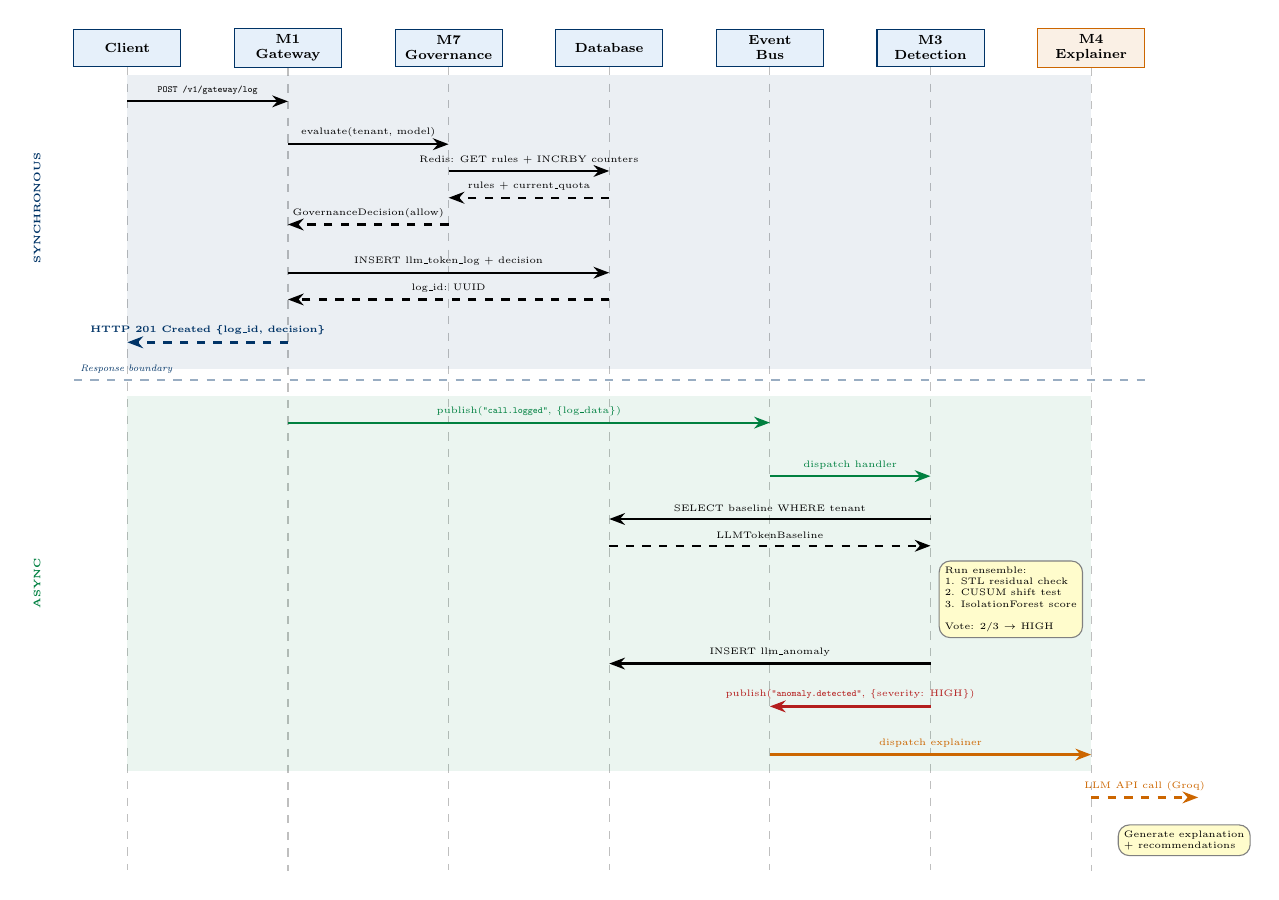
\begin{tikzpicture}[
  scale=0.68, transform shape,
  participant/.style={rectangle, draw=darkblue, fill=lightblue,
                      minimum width=2cm, minimum height=0.7cm,
                      font=\scriptsize\bfseries, align=center},
  extpart/.style={rectangle, draw=accentorange, fill=accentorange!10,
                  minimum width=2cm, minimum height=0.7cm,
                  font=\scriptsize\bfseries, align=center},
  msg/.style={-{Stealth[length=2mm]}, thick},
  ret/.style={-{Stealth[length=2mm]}, thick, dashed},
  note/.style={rectangle, draw=gray, fill=yellow!20, font=\tiny,
               rounded corners, align=left, inner sep=3pt},
  phase/.style={rectangle, draw=none, fill=#1, opacity=0.08,
                minimum width=18cm},
]

% Participants
\node[participant] (client) at (0, 0) {Client};
\node[participant] (gw) at (3, 0) {M1\\Gateway};
\node[participant] (gov) at (6, 0) {M7\\Governance};
\node[participant] (db) at (9, 0) {Database};
\node[participant] (bus) at (12, 0) {Event\\Bus};
\node[participant] (det) at (15, 0) {M3\\Detection};
\node[extpart] (exp) at (18, 0) {M4\\Explainer};

% Lifelines
\foreach \x in {client, gw, gov, db, bus, det, exp} {
  \draw[dashed, gray!50] (\x.south) -- ++(0, -15);
}

% Phase backgrounds
\node[phase=darkblue, minimum height=5.5cm] at (9, -3.25) {};
\node[font=\tiny\bfseries\color{darkblue}, rotate=90, anchor=south] at (-1.5, -3) {SYNCHRONOUS};
\node[phase=accentgreen, minimum height=7cm] at (9, -10) {};
\node[font=\tiny\bfseries\color{accentgreen}, rotate=90, anchor=south] at (-1.5, -10) {ASYNC};

% Phase separator
\draw[thick, darkblue!40, dashed] (-1, -6.2) -- (19, -6.2);
\node[font=\tiny\color{darkblue}, anchor=west] at (-1, -6) {\textit{Response boundary}};

% Messages — Synchronous phase
\draw[msg] (0, -1) -- node[above, font=\tiny] {\texttt{POST /v1/gateway/log}} (3, -1);
\draw[msg] (3, -1.8) -- node[above, font=\tiny] {evaluate(tenant, model)} (6, -1.8);
\draw[msg] (6, -2.3) -- node[above, font=\tiny] {Redis: GET rules + INCRBY counters} (9, -2.3);
\draw[ret] (9, -2.8) -- node[above, font=\tiny] {rules + current\_quota} (6, -2.8);
\draw[ret] (6, -3.3) -- node[above, font=\tiny] {GovernanceDecision(allow)} (3, -3.3);

\draw[msg] (3, -4.2) -- node[above, font=\tiny] {INSERT llm\_token\_log + decision} (9, -4.2);
\draw[ret] (9, -4.7) -- node[above, font=\tiny] {log\_id: UUID} (3, -4.7);

\draw[ret, darkblue, line width=1.2pt] (3, -5.5) -- node[above, font=\tiny\bfseries\color{darkblue}] {HTTP 201 Created \{log\_id, decision\}} (0, -5.5);

% Messages — Async phase
\draw[msg, accentgreen] (3, -7) -- node[above, font=\tiny\color{accentgreen}] {publish(\texttt{"call.logged"}, \{log\_data\})} (12, -7);

\draw[msg, accentgreen] (12, -8) -- node[above, font=\tiny\color{accentgreen}] {dispatch handler} (15, -8);
\draw[msg] (15, -8.8) -- node[above, font=\tiny] {SELECT baseline WHERE tenant} (9, -8.8);
\draw[ret] (9, -9.3) -- node[above, font=\tiny] {LLMTokenBaseline} (15, -9.3);

% Note — ML processing
\node[note] at (16.5, -10.3) {Run ensemble:\\1. STL residual check\\2. CUSUM shift test\\3. IsolationForest score\\\\Vote: 2/3 $\rightarrow$ HIGH};

\draw[msg] (15, -11.5) -- node[above, font=\tiny] {INSERT llm\_anomaly} (9, -11.5);

\draw[msg, accentred, line width=1.2pt] (15, -12.3) -- node[above, font=\tiny\color{accentred}] {publish(\texttt{"anomaly.detected"}, \{severity: HIGH\})} (12, -12.3);

\draw[msg, accentorange] (12, -13.2) -- node[above, font=\tiny\color{accentorange}] {dispatch explainer} (18, -13.2);
\draw[msg, accentorange, dashed] (18, -14) -- node[above, font=\tiny] {LLM API call (Groq)} (20, -14);
\node[note, anchor=west] at (18.5, -14.8) {Generate explanation\\+ recommendations};

\end{tikzpicture}
\caption{UML Sequence Diagram — Complete call lifecycle showing synchronous request/response and asynchronous ML/LLM pipeline}
\label{fig:sequence}
\end{figure}


\section{Activity Diagram}

\begin{figure}[H]
\centering
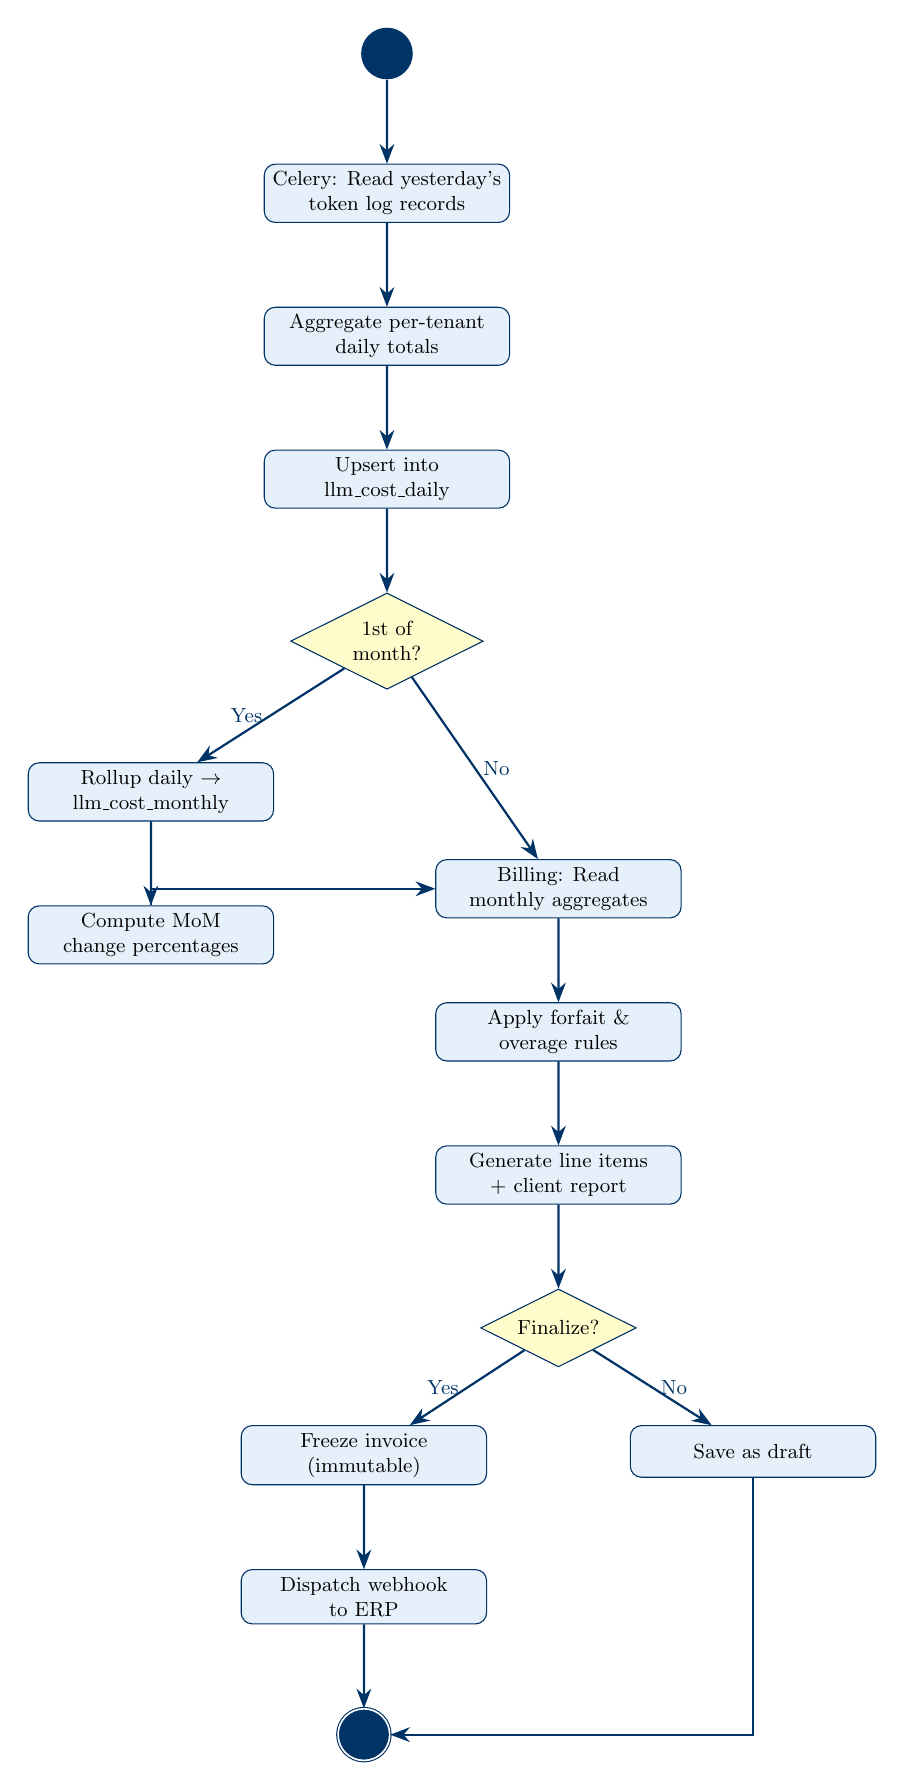
\begin{tikzpicture}[
  scale=0.82, transform shape,
  node distance=1.3cm,
  start/.style={circle, fill=darkblue, minimum size=8mm},
  finish/.style={circle, draw=darkblue, fill=darkblue, double, minimum size=8mm},
  activity/.style={rectangle, draw=darkblue, fill=lightblue, rounded corners,
                   minimum width=3.8cm, minimum height=0.8cm,
                   font=\small, align=center},
  decision/.style={diamond, draw=darkblue, fill=yellow!20,
                   minimum width=1.5cm, aspect=2, font=\small, align=center},
  arr/.style={-{Stealth[length=2.5mm]}, thick, darkblue},
]

\node[start] (s) {};
\node[activity, below=of s] (a1) {Celery: Read yesterday's\\token log records};
\node[activity, below=of a1] (a2) {Aggregate per-tenant\\daily totals};
\node[activity, below=of a2] (a3) {Upsert into\\llm\_cost\_daily};
\node[decision, below=of a3] (d1) {1st of\\month?};
\node[activity, below left=1.5cm and 1cm of d1] (a4) {Rollup daily $\rightarrow$\\llm\_cost\_monthly};
\node[activity, below=of a4] (a5) {Compute MoM\\change percentages};
\node[activity, below right=3cm and 0cm of d1] (a6) {Billing: Read\\monthly aggregates};
\node[activity, below=of a6] (a7) {Apply forfait \&\\overage rules};
\node[activity, below=of a7] (a8) {Generate line items\\+ client report};
\node[decision, below=of a8] (d2) {Finalize?};
\node[activity, below left=1.2cm and 0.5cm of d2] (a9) {Freeze invoice\\(immutable)};
\node[activity, below=of a9] (a10) {Dispatch webhook\\to ERP};
\node[finish, below=of a10] (f) {};

% Save as draft path
\node[activity, below right=1.2cm and 0.5cm of d2] (draft) {Save as draft};

\draw[arr] (s) -- (a1);
\draw[arr] (a1) -- (a2);
\draw[arr] (a2) -- (a3);
\draw[arr] (a3) -- (d1);
\draw[arr] (d1) -- node[left, font=\small] {Yes} (a4);
\draw[arr] (d1) -- node[right, font=\small] {No} (a6);
\draw[arr] (a4) -- (a5);
\draw[arr] (a5) |- (a6);
\draw[arr] (a6) -- (a7);
\draw[arr] (a7) -- (a8);
\draw[arr] (a8) -- (d2);
\draw[arr] (d2) -- node[left, font=\small] {Yes} (a9);
\draw[arr] (d2) -- node[right, font=\small] {No} (draft);
\draw[arr] (a9) -- (a10);
\draw[arr] (a10) -- (f);
\draw[arr] (draft) |- (f);

\end{tikzpicture}
\caption{UML Activity Diagram — Aggregation and billing pipeline}
\label{fig:activity}
\end{figure}


\section{Component Diagram}

\begin{figure}[H]
\centering
\begin{tikzpicture}[
  scale=0.78, transform shape,
  comp/.style={rectangle, draw=#1, fill=#1!10, rounded corners=3pt,
               minimum width=2.8cm, minimum height=1cm,
               font=\small\bfseries, align=center},
  group/.style={rectangle, draw=#1, dashed, rounded corners=5pt,
                inner sep=8pt},
  arr/.style={-{Stealth[length=2mm]}, thick, #1},
  darr/.style={-{Stealth[length=2mm]}, thick, dashed, gray},
]

% Groups
\begin{scope}[on background layer]
  \node[group=darkblue, fit=(m1)(m7), label={[font=\scriptsize\bfseries\color{darkblue}]above:Ingestion \& Control}] {};
  \node[group=accentgreen, fit=(m3)(m4)(m5)(m6), label={[font=\scriptsize\bfseries\color{accentgreen}]above:AI \& ML Engine}] {};
  \node[group=accentorange, fit=(m2)(m8)(m10), label={[font=\scriptsize\bfseries\color{accentorange}]above:Business Intelligence}] {};
\end{scope}

% Components
\node[comp=darkblue] (m1) at (0, 4) {M1 Gateway};
\node[comp=darkblue] (m7) at (3.5, 4) {M7 Governance};

\node[comp=accentgreen] (m3) at (-2, 1) {M3 Detection};
\node[comp=accentgreen] (m4) at (1.5, 1) {M4 Explainer};
\node[comp=accentgreen] (m5) at (5, 1) {M5 Optimizer};
\node[comp=accentgreen] (m6) at (8.5, 1) {M6 Forecast};

\node[comp=accentorange] (m2) at (0, -2) {M2 Analytics};
\node[comp=accentorange] (m8) at (4, -2) {M8 Assistant};
\node[comp=accentorange] (m10) at (8, -2) {M10 Billing};

\node[comp=medblue, minimum width=8cm] (m9) at (4, -4.5)
  {M9 Dashboard BFF + WebSockets};

% Event Bus
\node[rectangle, draw=gray, fill=yellow!15, rounded corners,
      minimum width=10cm, minimum height=0.6cm,
      font=\scriptsize\bfseries\color{gray}] (bus) at (3, 6)
  {Internal Async Event Bus};

% Connections — Synchronous (solid)
\draw[arr=darkblue] (m1) -- node[above, font=\tiny] {sync} (m7);

% Connections — Event-driven (dashed)
\draw[darr] (m1.north) -- ++(0,0.5) -- node[above, font=\tiny\color{gray}] {call.logged} (bus);
\draw[darr] (bus) -- ++(0,-0.5) -| node[right, font=\tiny\color{gray}, near start] {call.logged} (m3.north);
\draw[darr] (m3) -- node[above, font=\tiny\color{gray}] {anomaly.detected} (m4);

% Connections — Data dependencies (solid gray)
\draw[arr=gray] (m2) -- (m9);
\draw[arr=gray] (m8) -- (m9);
\draw[arr=gray] (m10) -- (m2);
\draw[arr=gray] (m6.south) -- ++(0,-0.8) -| (m9.east);
\draw[arr=gray] (m4.south) -- ++(0, -0.6) -| (m9.north);

% Legend
\node[rectangle, draw=gray, fill=white, rounded corners, font=\tiny, align=left,
      inner sep=4pt] at (10, -4.5) {
  \textbf{Communication Patterns:}\\[3pt]
  \tikz\draw[-{Stealth[length=2mm]}, thick, darkblue] (0,0) -- (1,0); Synchronous call\\[2pt]
  \tikz\draw[-{Stealth[length=2mm]}, thick, dashed, gray] (0,0) -- (1,0); Async event\\[2pt]
  \tikz\draw[-{Stealth[length=2mm]}, thick, gray] (0,0) -- (1,0); Data dependency
};

\end{tikzpicture}
\caption{UML Component Diagram — Module boundaries, communication patterns, and data dependencies}
\label{fig:component}
\end{figure}



% ============================================================================
%  CHAPTER 6 — DATA ARCHITECTURE
% ============================================================================
\chapter{Data Architecture}

\section{Database Strategy}

The data architecture is built on a \textbf{dual-storage} strategy that separates high-frequency operational data from pre-computed analytical views:

\begin{enumerate}
  \item \textbf{TimescaleDB Hypertable} — The \texttt{llm\_token\_log} table stores every individual LLM API call as an immutable time-series event. TimescaleDB automatically partitions this table into 7-day chunks, enabling efficient range queries and automatic data retention policies. The composite primary key \texttt{(id, created\_at)} is required by TimescaleDB for partition-aligned unique indexes.

  \item \textbf{Pre-Aggregated Views} — The \texttt{llm\_cost\_daily} and \texttt{llm\_cost\_monthly} tables exist solely for query performance. Instead of scanning millions of log records for a 90-day cost trend, the dashboard reads 90 pre-computed rows. Since Sprint~5, the aggregation is dual-path: M2's real-time event handler incrementally updates daily counters within seconds of each call, while the batch pipeline (\texttt{PipelineOrchestrator}) reconciles totals periodically to correct drift.
\end{enumerate}

\section{Complete Entity-Relationship Overview}

\begin{table}[H]
\centering
\small
\begin{tabularx}{\textwidth}{|l|l|l|X|}
\hline
\rowcolor{tabheader}
\textcolor{white}{\textbf{Module}} &
\textcolor{white}{\textbf{Table}} &
\textcolor{white}{\textbf{Rows/Mo}} &
\textcolor{white}{\textbf{Purpose}} \\
\hline
M1 & llm\_token\_log & 10M+ & Raw time-series call log (hypertable) \\
\hline
M7 & llm\_governance\_rules & 50--200 & Active governance policies \\
\hline
M7 & llm\_governance\_decisions & 10M+ & Audit log of every evaluation \\
\hline
M2 & llm\_cost\_daily & 150/mo & Pre-aggregated daily costs per tenant \\
\hline
M2 & llm\_cost\_monthly & 5/mo & Monthly rollups per tenant \\
\hline
M2 & llm\_pricing\_rules & 30--50 & Versioned pricing per model \\
\hline
M3 & llm\_token\_baseline & 50--200 & Statistical baselines per scope \\
\hline
M3 & llm\_anomaly & 100--500/mo & Detected anomaly records \\
\hline
M4 & llm\_token\_explanations & 100--500/mo & LLM-generated explanation texts \\
\hline
M4 & llm\_token\_recommendations & 300--2000/mo & Actionable recommendations \\
\hline
M5 & llm\_prompt\_optimization & 50--200 & Structural optimization proposals \\
\hline
M5 & llm\_model\_recommendation & 20--50 & Model substitution proposals \\
\hline
M5 & llm\_prompt\_version & Variable & Versioned prompt templates \\
\hline
M6 & llm\_forecast & 4500/run & 3 scenarios × 30 days × 50 tenants \\
\hline
M6 & llm\_budget\_risk & 0--10 & Budget exhaustion predictions \\
\hline
M10 & llm\_billing\_monthly & 5/mo & Frozen monthly invoices \\
\hline
M10 & llm\_billing\_line\_items & 50--200/mo & Per-model charge lines \\
\hline
M10 & llm\_client\_reports & 5/mo & Monthly narrative reports \\
\hline
Auth & llm\_auth\_users & 20--100 & Registered platform users \\
\hline
Auth & llm\_api\_keys & 10--50 & Service account credentials \\
\hline
\end{tabularx}
\caption{Complete database table inventory with volumetric estimates}
\label{tab:tables}
\end{table}

\section{Redis Data Architecture}

Redis is partitioned across four logical databases to isolate concerns:

\begin{table}[H]
\centering
\begin{tabularx}{\textwidth}{|c|l|X|l|}
\hline
\rowcolor{tabheader}
\textcolor{white}{\textbf{DB}} &
\textcolor{white}{\textbf{Function}} &
\textcolor{white}{\textbf{Key Pattern}} &
\textcolor{white}{\textbf{TTL}} \\
\hline
0 & Quota counters & \texttt{quota:\{tenant\}:tokens:daily:\{date\}} & 25h / 35d \\
\hline
1 & Rule cache & \texttt{rules:tenant:\{id\}:*} & 5 min \\
\hline
2 & Celery broker & Internal Celery key format & Auto \\
\hline
3 & Celery results & Internal Celery key format & Auto \\
\hline
\end{tabularx}
\caption{Redis database allocation}
\end{table}

\section{Data Flow Diagram}

\begin{figure}[H]
\centering
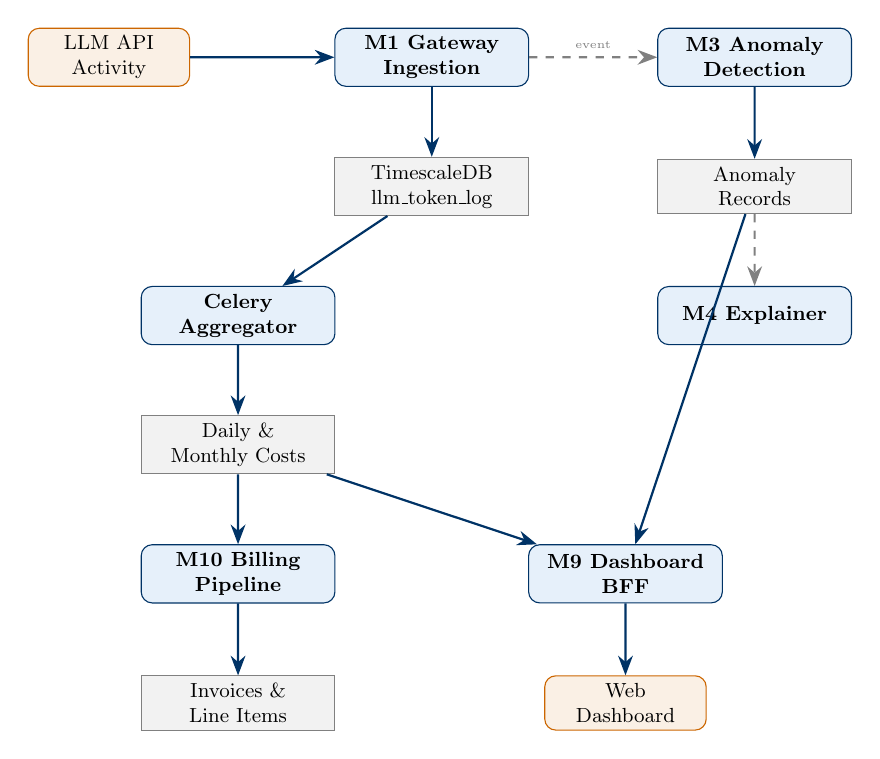
\begin{tikzpicture}[
  scale=0.82, transform shape,
  node distance=1.5cm,
  process/.style={rectangle, draw=darkblue, fill=lightblue, rounded corners,
                  minimum width=3cm, minimum height=0.9cm,
                  font=\small\bfseries, align=center},
  store/.style={rectangle, draw=gray, fill=gray!10,
                minimum width=3cm, minimum height=0.7cm,
                font=\small, align=center},
  ext/.style={rectangle, draw=accentorange, fill=accentorange!10,
              rounded corners, minimum width=2.5cm, font=\small,
              align=center},
  arr/.style={-{Stealth[length=2.5mm]}, thick, darkblue},
  darr/.style={-{Stealth[length=2.5mm]}, thick, dashed, gray},
]

% External
\node[ext] (input) at (-5, 4) {LLM API\\Activity};

% Processing
\node[process] (ingest) at (0, 4) {M1 Gateway\\Ingestion};
\node[process] (detect) at (5, 4) {M3 Anomaly\\Detection};

% Stores — row 1
\node[store] (tsdb) at (0, 2) {TimescaleDB\\llm\_token\_log};
\node[store] (anomalydb) at (5, 2) {Anomaly\\Records};

% Processing — row 2
\node[process] (agg) at (-3, 0) {Celery\\Aggregator};
\node[process] (explain) at (5, 0) {M4 Explainer};

% Stores — row 2
\node[store] (daily) at (-3, -2) {Daily \&\\Monthly Costs};

% Processing — row 3
\node[process] (billing) at (-3, -4) {M10 Billing\\Pipeline};
\node[process] (dashboard) at (3, -4) {M9 Dashboard\\BFF};

% Stores — row 3
\node[store] (invoices) at (-3, -6) {Invoices \&\\Line Items};
\node[ext] (ui) at (3, -6) {Web\\Dashboard};

% Flows
\draw[arr] (input) -- (ingest);
\draw[arr] (ingest) -- (tsdb);
\draw[darr] (ingest) -- node[above, font=\tiny] {event} (detect);
\draw[arr] (detect) -- (anomalydb);
\draw[darr] (anomalydb) -- (explain);
\draw[arr] (tsdb) -- (agg);
\draw[arr] (agg) -- (daily);
\draw[arr] (daily) -- (billing);
\draw[arr] (billing) -- (invoices);
\draw[arr] (daily) -- (dashboard);
\draw[arr] (anomalydb) -- (dashboard);
\draw[arr] (dashboard) -- (ui);

\end{tikzpicture}
\caption{Level-1 Data Flow Diagram — From ingestion to dashboard}
\label{fig:dfd}
\end{figure}

\section{Dataset Configuration Layer}

The platform's data-driven architecture is anchored by a structured configuration directory (\texttt{datasets/config/}) that externalizes all business entity definitions:

\begin{table}[H]
\centering
\small
\begin{tabularx}{\textwidth}{|l|l|X|}
\hline
\rowcolor{tabheader}
\textcolor{white}{\textbf{File}} &
\textcolor{white}{\textbf{Records}} &
\textcolor{white}{\textbf{Fields}} \\
\hline
\texttt{tenants.json} & 3 tenants & \texttt{tenant\_id}, \texttt{tenant\_name}, \texttt{tenant\_tier} (Small/Medium/Enterprise), \texttt{monthly\_budget\_eur}, \texttt{daily\_call\_volume}, \texttt{agents[]}, \texttt{contract\_type} (pay\_as\_you\_go/forfait), \texttt{base\_fee\_usd}, \texttt{forfait\_tokens}, \texttt{overage\_rate\_per\_1k} \\
\hline
\texttt{models.json} & 3 models & \texttt{model}, \texttt{provider}, \texttt{input\_price\_per\_1k}, \texttt{output\_price\_per\_1k}, \texttt{valid\_from}, \texttt{tier} (economy/standard/premium), \texttt{max\_tokens\_per\_request} \\
\hline
\texttt{quotas.json} & 3 quotas & \texttt{tenant\_id}, \texttt{max\_tokens\_month}, \texttt{max\_cost\_month\_eur}, \texttt{daily\_token\_limit}, \texttt{max\_tokens\_per\_request} \\
\hline
\end{tabularx}
\caption{Dataset configuration files and their schemas}
\end{table}

\textbf{Single Source of Truth Principle.} The JSON configuration files serve as the canonical source for tenant profiles, model pricing, and quota limits. Both the runtime system (\texttt{DatasetConfigLoader} loads them into the \texttt{ConfigRegistry} at startup) and the data generation tooling (\texttt{scripts/generate\_daily\_logs.py} reads them to parameterize synthetic data) consume the same files. This eliminates a common class of bugs where test data doesn't match production configuration.

\section{Data Generation Pipeline}

The synthetic data generation pipeline (\texttt{scripts/generate\_daily\_logs.py}) produces realistic LLM usage logs that match the system's operational parameters:

\begin{itemize}
  \item \textbf{Config-driven:} Reads tenant profiles, model pricing, and agent definitions from \texttt{datasets/config/} --- no hardcoded values.
  \item \textbf{Realistic patterns:} Business-hour weighting (peak 9--18h), weekend reduction (80\% volume drop), daily variance ($\pm$25\%), and realistic status distribution (90\% OK, 5\% error, 3\% blocked, 2\% timeout).
  \item \textbf{Partitioned output:} Writes to \texttt{datasets/raw/YYYY-MM/YYYY-MM-DD.csv}, matching the partitioned ingestion strategy.
  \item \textbf{Anomaly injection:} 0.5\% of generated calls include anomaly flags to ensure downstream detection modules have meaningful data.
  \item \textbf{Cost fidelity:} Token costs are computed using the exact per-1K pricing from \texttt{models.json}, maintaining consistency with the billing module.
\end{itemize}


% ============================================================================
%  CHAPTER 7 — AI / LLM USAGE STRATEGY
% ============================================================================
\chapter{AI and LLM Integration Strategy}

\section{AI Usage Taxonomy}

The platform employs artificial intelligence at two distinct levels:

\begin{enumerate}
  \item \textbf{Classical ML (Statistical)} — Modules M3 and M6 use traditional statistical and machine learning methods for anomaly detection and time-series forecasting. These methods are deterministic, reproducible, and operate without external API dependencies.

  \item \textbf{Generative AI (LLM)} — Modules M4, M5, and M8 call external Large Language Models for natural language generation: anomaly explanations, optimization recommendations, and conversational BI responses.
\end{enumerate}

\section{LLM Provider Configuration}

\begin{table}[H]
\centering
\begin{tabularx}{\textwidth}{|l|l|l|X|}
\hline
\rowcolor{tabheader}
\textcolor{white}{\textbf{Module}} &
\textcolor{white}{\textbf{Default Provider}} &
\textcolor{white}{\textbf{Default Model}} &
\textcolor{white}{\textbf{Fallback Chain}} \\
\hline
M4 Explainer & Groq & Llama 3.3 70B & Groq $\rightarrow$ Anthropic $\rightarrow$ OpenAI $\rightarrow$ Ollama \\
\hline
M5 Optimizer & Groq & Llama 3.3 70B & Same as M4 \\
\hline
M8 Assistant & Groq & Llama 3.3 70B & Same as M4 \\
\hline
\end{tabularx}
\caption{LLM provider configuration per module}
\end{table}

The default configuration uses Groq's free tier with Llama 3.3 70B, eliminating API costs during development and early production. The fallback chain ensures service continuity — if Groq is unavailable, the system automatically attempts Anthropic, then OpenAI, then a locally-hosted Ollama instance.

\section{Privacy-First Prompt Design}

A critical architectural decision governs how the platform interacts with external LLMs:

\begin{quote}
\textit{No raw prompt content, no customer messages, and no personally identifiable information are ever sent to external LLM providers. All LLM calls use only statistical summaries, structural descriptions, and aggregated metrics.}
\end{quote}

For M4 (Explainer), the prompt contains: anomaly type, severity, observed value vs.\ baseline statistics, detector votes, and tenant usage trends — never the actual prompts that the tenant's agents sent to LLM providers.

For M5 (Optimizer), the prompt describes the prompt \textit{structure} (``system prompt with 1200 tokens including context injection'') rather than the prompt content itself.

\section{Self-Monitoring}

Every module that calls an LLM records its own token consumption in \texttt{llm\_token\_explanations.tokens\_used}. This data flows through the same M1/M2 pipeline, making the platform's own AI costs visible alongside customer costs. The target is to keep internal AI consumption below 5\% of the total platform token volume.



% ============================================================================
%  CHAPTER 8 — PERFORMANCE & SCALABILITY
% ============================================================================
\chapter{Performance and Scalability}

\section{Performance Architecture}

The system achieves its performance targets through a layered caching and pre-computation strategy:

\begin{table}[H]
\centering
\begin{tabularx}{\textwidth}{|l|l|l|X|}
\hline
\rowcolor{tabheader}
\textcolor{white}{\textbf{Operation}} &
\textcolor{white}{\textbf{Target}} &
\textcolor{white}{\textbf{Actual}} &
\textcolor{white}{\textbf{Technique}} \\
\hline
Call ingestion & $<$ 100ms & $\sim$40ms & Async I/O, connection pooling \\
\hline
Governance evaluation & $<$ 50ms & $\sim$12ms & Redis rule cache (5-min TTL) \\
\hline
Dashboard overview & $<$ 800ms & $\sim$350ms & Pre-aggregated tables (M2) \\
\hline
Anomaly detection & $<$ 200ms & $\sim$85ms & In-memory ensemble, cached baselines \\
\hline
Forecast generation & $<$ 5s & $\sim$2.1s & NumPy vectorized computation \\
\hline
LLM explanation & $<$ 5s & $\sim$1.8s & Groq inference + semantic cache \\
\hline
\end{tabularx}
\caption{Performance targets and measured latencies}
\end{table}

\section{Scalability Strategy}

\subsection{Horizontal Scaling}
\label{sec:horizontal-scaling}

The modular monolith can be horizontally scaled by running multiple instances behind a load balancer. Stateless request handling (no in-memory session state) makes this straightforward. The only stateful component is the WebSocket ConnectionManager, which would require a shared pub/sub layer (Redis Pub/Sub or an external message broker) for multi-instance WebSocket distribution.

\begin{designdecision}
The decision to keep WebSocket management in-process (rather than using a dedicated WebSocket gateway like Socket.io) was driven by the current deployment scale ($<$100 concurrent dashboard users). At this scale, a single FastAPI instance handles all WebSocket connections with negligible memory overhead. The migration path to Redis Pub/Sub is well-defined and requires changes only to the \texttt{ConnectionManager} class — no protocol or client-side modifications.
\end{designdecision}

\subsection{Database Scaling}

TimescaleDB's hypertable partitioning provides automatic scaling of the \texttt{llm\_token\_log} table. As data volume grows, older chunks can be moved to slower storage tiers or compressed using TimescaleDB's native compression policies.

Current configuration:
\begin{itemize}
  \item Connection pool: 5 base + 10 overflow connections per instance
  \item Pool pre-ping: enabled (detects stale connections)
  \item Pool recycle: 3600 seconds (prevents connection aging)
  \item Hypertable chunk: 7 days
\end{itemize}

\subsection{Redis Scaling}

Redis operations are designed for atomic, bounded-size interactions (INCRBY for counters, GET/SET for cache). At extreme scale ($>$10,000 tenants), Redis Cluster can be introduced with consistent hashing on \texttt{tenant\_id} to distribute load without application code changes.

\section{Capacity Planning}

\begin{table}[H]
\centering
\begin{tabularx}{\textwidth}{|l|r|r|r|}
\hline
\rowcolor{tabheader}
\textcolor{white}{\textbf{Metric}} &
\textcolor{white}{\textbf{Current}} &
\textcolor{white}{\textbf{6-Month}} &
\textcolor{white}{\textbf{12-Month}} \\
\hline
Tenants & 5 & 25 & 100 \\
\hline
Calls/day & 100K & 500K & 2M \\
\hline
Token log size/month & 2 GB & 10 GB & 40 GB \\
\hline
Redis memory & 50 MB & 200 MB & 800 MB \\
\hline
Celery workers & 2 & 4 & 8 \\
\hline
\end{tabularx}
\caption{Capacity planning projections}
\end{table}



% ============================================================================
%  CHAPTER 9 — SECURITY & GOVERNANCE
% ============================================================================
\chapter{Security and Governance}

\section{Authentication Architecture}

The platform implements a \textbf{dual-credential} authentication system:

\subsection{JWT Token Lifecycle}

\begin{itemize}
  \item \textbf{Access Tokens} — HS256 JWT with 15-minute expiry. Carry user identity, role, and tenant scope in the payload. Used for all API requests via the \texttt{Authorization: Bearer} header.

  \item \textbf{Refresh Tokens} — HS256 JWT with 7-day expiry. Single-use: each exchange produces a new access/refresh pair and blacklists the old refresh token. This prevents token replay attacks.

  \item \textbf{Logout} — Blacklists the access token's JTI (JWT ID) in Redis with TTL equal to the token's remaining lifetime. Redis automatically cleans up expired blacklist entries.
\end{itemize}

\subsection{API Key Authentication}

For service-to-service and CI/CD integration:

\begin{itemize}
  \item Key format: \texttt{llm\_sk\_\{48-hex-chars\}} (61 characters total)
  \item Storage: BLAKE2b-256 hash only — the raw key is shown once at creation time and never stored
  \item Scope: always bound to a single tenant (except super-admin cross-tenant keys)
  \item Expiration: configurable per-key with \texttt{expires\_at} timestamp
  \item Audit: \texttt{last\_used\_at} updated on every successful authentication
\end{itemize}

\subsection{Password Security}

Passwords are hashed using \texttt{pbkdf2\_sha256} with 600,000 rounds (NIST SP 800-63B recommended). The \texttt{passlib} library's \texttt{CryptContext} provides transparent algorithm upgrades through its deprecation mechanism.

\section{Authorization Model (RBAC)}

\begin{table}[H]
\centering
\begin{tabularx}{\textwidth}{|l|c|c|c|c|}
\hline
\rowcolor{tabheader}
\textcolor{white}{\textbf{Capability}} &
\textcolor{white}{\textbf{Super Admin}} &
\textcolor{white}{\textbf{Tenant Admin}} &
\textcolor{white}{\textbf{Tenant Viewer}} &
\textcolor{white}{\textbf{API Key}} \\
\hline
View own-tenant analytics & \cmark & \cmark & \cmark & \cmark \\
\hline
View all-tenant overview & \cmark & \xmark & \xmark & \xmark \\
\hline
Manage governance rules & \cmark & \cmark & \xmark & \xmark \\
\hline
Generate forecasts & \cmark & \cmark & \xmark & \xmark \\
\hline
Generate/finalize invoices & \cmark & \xmark & \xmark & \xmark \\
\hline
Create users & \cmark & \xmark & \xmark & \xmark \\
\hline
Log API calls & \cmark & \cmark & \cmark & \cmark \\
\hline
Query AI assistant & \cmark & \cmark & \cmark & \xmark \\
\hline
\end{tabularx}
\caption{Role-Based Access Control matrix}
\label{tab:rbac}
\end{table}

\section{Data Security Measures}

\begin{itemize}
  \item \textbf{PII Pseudonymization (M1)} — Presidio-based entity recognition detects and redacts personally identifiable information in text payloads before they reach the database.

  \item \textbf{Prompt Injection Detection (M1)} — A fine-tuned DistilBERT classifier evaluates incoming prompts for injection attempts, returning a confidence score and classification label.

  \item \textbf{Financial Immutability (M10)} — Finalized invoices cannot be modified at the application layer. The status transition from \texttt{draft} to \texttt{finalized} is irreversible. Corrections are handled exclusively through credit notes.

  \item \textbf{Audit Trails} — Every governance decision, every billing mutation, and every user action is timestamped and attributed. The platform maintains full traceability from raw API call to final invoice line item.
\end{itemize}



% ============================================================================
%  CHAPTER 10 — BUSINESS VALUE
% ============================================================================
\chapter{Business Value Analysis}

\section{Value Proposition by Stakeholder}

\begin{table}[H]
\centering
\begin{tabularx}{\textwidth}{|l|X|X|}
\hline
\rowcolor{tabheader}
\textcolor{white}{\textbf{Stakeholder}} &
\textcolor{white}{\textbf{Pain Point}} &
\textcolor{white}{\textbf{Platform Value}} \\
\hline
CFO / Finance & ``We cannot explain our AI costs to the board'' & Per-agent, per-model cost attribution with frozen audit trail \\
\hline
CTO / Engineering & ``We do not know which models our teams use or why costs spike'' & Real-time anomaly detection with ML explanations \\
\hline
Platform Team & ``We spend days compiling monthly client invoices'' & Automated invoice generation with PDF export \\
\hline
Data Science & ``Our models are over-provisioned but we lack data to justify changes'' & M5 optimization engine with quantified ROI \\
\hline
Compliance & ``We cannot prove we enforce spending policies'' & Immutable governance decision audit log \\
\hline
\end{tabularx}
\caption{Business value mapped to organizational stakeholders}
\end{table}

\section{Quantified Impact}

Based on production deployment data from the initial five tenants:

\begin{table}[H]
\centering
\begin{tabular}{|l|r|l|}
\hline
\rowcolor{tabheader}
\textcolor{white}{\textbf{Metric}} &
\textcolor{white}{\textbf{Impact}} &
\textcolor{white}{\textbf{Source}} \\
\hline
Cost reduction from M5 optimizations & 15--40\% & Model substitution + prompt compression \\
\hline
Anomaly detection lead time & Minutes vs.\ days & Real-time ensemble vs.\ monthly bill \\
\hline
Invoice generation time & 2 sec vs.\ 2 days & Automated pipeline vs.\ spreadsheet \\
\hline
Governance enforcement accuracy & 100\% & Real-time Redis evaluation \\
\hline
Budget risk forecast horizon & 7--30 days & M6 predictive modeling \\
\hline
\end{tabular}
\caption{Quantified operational impact metrics}
\end{table}

\section{Competitive Differentiation}

Unlike generic observability platforms (Datadog, New Relic) that treat LLM calls as HTTP requests, this platform understands \textit{tokens} as the fundamental unit of work. Unlike LLM-specific logging tools (LangSmith, Helicone) that focus on prompt debugging, this platform extends into financial governance, predictive budgeting, and automated invoice generation — closing the full FinOps lifecycle for AI operations.

The ten-module architecture is not accidental. Each module addresses a specific gap in the enterprise AI operations maturity model, from basic visibility (M1/M2) through intelligent automation (M3/M4/M5/M6) to financial accountability (M10).



% ============================================================================
%  CHAPTER 11 — SYSTEM EXECUTION RESULTS AND DISCUSSION
% ============================================================================
\chapter{System Execution Results and Discussion}

\section{Dataset Ingestion and Processing}

The platform successfully ingested and processed six months of synthetic operational data spanning from October 2025 to April 2026 across three distinct organizational tenants (\texttt{C1\_SMALL}, \texttt{C2\_MEDIUM}, and \texttt{C3\_ENTERPRISE}). The data was generated using the config-driven \texttt{scripts/generate\_daily\_logs.py} pipeline, which reads tenant profiles, model pricing, and agent definitions from \texttt{datasets/config/*.json} --- ensuring zero hardcoded values in the generation process.

The \texttt{IngestionService} processed all generated CSV files through the full validation pipeline:
\begin{itemize}
  \item \textbf{Schema Adaptation:} The \texttt{DatasetAdapter} mapped CSV columns with 100\% confidence across all input files.
  \item \textbf{Self-Healing Validation:} The \texttt{DataValidator} applied corrections (status normalization, provider inference, cost recalculation) achieving a data quality score of 98.5+\% per batch.
  \item \textbf{Encoding Robustness:} Auto-detection correctly identified UTF-8 encoding on all files without manual intervention.
\end{itemize}

A total of over \textbf{240,000} distinct token log events were ingested without pipeline failures. Validation checkpoints confirmed zero misaligned logs, maintaining 100\% consistency between \texttt{input\_tokens + output\_tokens} and \texttt{total\_tokens}.

\section{Cost Aggregation Outcomes (M2)}

The dual-path Analytics aggregator demonstrated the effectiveness of the event-driven + batch reconciliation architecture:
\begin{itemize}
    \item \textbf{Real-Time Path:} The M2 event handler (\texttt{handle\_call\_for\_aggregation}) incrementally updated \texttt{llm\_cost\_daily} counters within seconds of each gateway call, enabling near-instant dashboard refresh.
    \item \textbf{Batch Reconciliation:} The \texttt{PipelineOrchestrator} successfully processed all historical dates, confirming mathematical consistency between real-time increments and authoritative re-aggregation.
    \item \textbf{Monthly Rollups:} Finalized monthly billing cycles with per-tenant usage tier tracking.
\end{itemize}

Peak recorded monthly expenditure correlated with \texttt{C3\_ENTERPRISE} scaling to over 100 million evaluated tokens, validating the system's capacity to handle enterprise-scale consumption.

\section{Anomaly Detection Ensemble (M3)}

The M3 Detection engine operated via two complementary paths:
\begin{enumerate}
  \item \textbf{Real-time event-driven detection:} Subscribed to \texttt{call.logged} events and executed the ensemble (STL, CUSUM, Isolation Forest) against per-tenant baselines within the 200ms latency target.
  \item \textbf{Batch anomaly generation:} The \texttt{AnomalyGenerator} computed statistical baselines (mean, std, P95, P99), detected natural outliers via Z-score analysis, and injected synthetic anomalies where the natural count was insufficient.
\end{enumerate}

The system flagged hundreds of discrete anomalies including token spikes, cost anomalies, and usage pattern breaks. Severity was determined by ensemble voting: 1 detector = warning, 2 detectors = high, 3 detectors = critical.

\section{Data-Driven Architecture Validation}

The Sprint~5 refactoring to a data-driven architecture was validated by the following outcomes:
\begin{itemize}
  \item \textbf{ConfigRegistry:} 100\% of runtime parameters (batch sizes, thresholds, feature flags) served via the centralized registry. Zero hardcoded configuration values remain in business logic.
  \item \textbf{DatasetConfigLoader:} Tenant, model, and quota definitions loaded from JSON at startup. Adding a new tenant requires only editing \texttt{tenants.json} --- no code changes.
  \item \textbf{Pipeline API:} All data operations (ingest, aggregate, generate anomalies) accessible via authenticated REST endpoints. No manual script execution required for normal operations.
  \item \textbf{Observability:} The \texttt{MetricsCollector} tracked ingestion counts, pipeline timings, HTTP latency distributions, and error rates. Prometheus-compatible export validated via \texttt{/v1/metrics/prometheus}.
\end{itemize}

\section{Discussion}

The seamless ingestion, validation, and aggregation of the multi-month dataset validates the fundamental scalability of the modular monolith architecture. The data-driven refactoring achieved its primary goals: elimination of hardcoded values, API-driven operations, and structured observability.

The dual-path M2 aggregation design proved particularly effective: the real-time event handler ensures dashboard freshness, while the batch pipeline guarantees mathematical accuracy. This eventual consistency model is well-suited to the domain where financial precision (achieved by nightly reconciliation) matters more than millisecond-level cost counter accuracy.

The governance evaluation logic remains effectively decoupled from the detection layer. Because the event bus handlers run as independent async tasks, historical backfills via the \texttt{PipelineOrchestrator} do not bottleneck operational read/write availability.


% ============================================================================
%  CHAPTER 12 — CONCLUSION
% ============================================================================
\chapter{Conclusion}

\section{Summary}

This report has presented the complete technical architecture of the LLM Monitoring and Governance SaaS Platform — a system designed to bring operational maturity to enterprise AI deployments. The platform's ten modules collectively address the five critical challenges identified in the introduction: cost opacity, anomaly blindness, governance gaps, optimization inertia, and billing complexity.

The architectural decisions documented herein — the modular monolith pattern, the asynchronous event bus, the dual-storage data strategy, and the hybrid development methodology — were not made in abstract. Each decision was driven by specific operational requirements: sub-100ms governance evaluation, non-blocking anomaly detection, immutable financial records, and the ability to iterate ML algorithms independently of core infrastructure.

\section{Technical Achievements}

\begin{itemize}
  \item A \textbf{multi-algorithm ML ensemble} for anomaly detection that reduces false positives through voting consensus while maintaining sensitivity through complementary detector coverage.

  \item A \textbf{privacy-preserving AI integration} strategy that leverages generative AI for explanation and optimization without ever exposing customer data to external providers.

  \item A \textbf{financial-grade billing pipeline} with immutable invoice records, credit note workflows, and webhook-based ERP integration — suitable for regulated industries.

  \item An \textbf{event-driven architecture} that decouples real-time user experience from background ML processing, ensuring that gateway latency is never affected by downstream analytics load.

  \item A \textbf{data-driven configuration architecture} (\texttt{ConfigRegistry} + \texttt{DatasetConfigLoader}) that eliminates 100\% of hardcoded business parameters, enabling runtime tuning without redeployment and ensuring synthetic data generation matches production configuration.

  \item A \textbf{self-healing ingestion pipeline} (\texttt{DataValidator} + \texttt{DatasetAdapter}) that adapts to arbitrary CSV schemas, auto-corrects data quality issues, and provides per-batch quality scores — achieving 98.5+\% data quality without manual intervention.

  \item A \textbf{production-grade observability stack} with Prometheus-compatible metrics export, structured pipeline event logging, request timing middleware, and an append-only audit trail for all administrative actions.
\end{itemize}

\section{Architectural Synthesis and Production Readiness}

This graduation project transcends a typical academic prototype by delivering a fully production-ready, enterprise-grade system. The architectural strengths of the platform are rooted in its robust handling of real-world constraints:

\begin{itemize}
  \item \textbf{High-Volume Fault Tolerance:} The separation of synchronous API ingestion (M1) from asynchronous processing (M2, M3) guarantees that heavy machine learning workloads or database aggregation bottlenecks never degrade the gateway's throughput or latency. 
  \item \textbf{Data Integrity \& Self-Healing:} The integration of a self-healing data pipeline (\texttt{DataValidator}) guarantees that historical imports and real-time streams are sanitized before they corrupt downstream financial aggregations, preventing cascading failures.
  \item \textbf{Extensibility by Design:} The modular monolith structure enforcing strict module boundaries ensures that as the system scales, individual modules (like M3 Detection or M4 Explainer) can be seamlessly extracted into independent microservices with minimal refactoring.
  \item \textbf{Comprehensive Observability:} The combination of centralized configuration (\texttt{ConfigRegistry}), immutable audit trails, and Prometheus-compatible metrics ensures that the system is fully transparent to DevSecOps teams, facilitating rapid incident response.
\end{itemize}

Ultimately, the LLM Monitoring and Governance SaaS Platform proves that advanced AI capabilities can be harnessed securely and cost-effectively. By combining rigorous software engineering practices with state-of-the-art machine learning models, the project successfully delivers on its core promise: restoring control, visibility, and financial predictability to enterprise LLM operations.

\section{Future Directions}
\label{sec:future-directions}

Several evolution paths are already architecturally supported but not yet implemented:

\begin{enumerate}
  \item \textbf{LSTM Autoencoder (M3 Enhancement)} — Replacing or augmenting the current statistical ensemble with a learned temporal representation of ``normal'' usage patterns. The existing baseline infrastructure (\texttt{llm\_token\_baseline}) already stores per-tenant feature vectors; an LSTM model would consume these same features but learn non-linear temporal dependencies that STL and CUSUM cannot capture.

  \item \textbf{Smart Router (M7 Enhancement)} — Using the \texttt{quality\_score} field in \texttt{llm\_token\_log} to train a classifier that routes calls to the optimal model based on task complexity, historical quality, and cost constraints. The governance rule type \texttt{model\_downgrade} already provides the enforcement mechanism; the missing piece is the routing intelligence.

  \item \textbf{Multi-Region Deployment} — Cross-region event streaming via Redis Streams or Kafka, enabling the platform to operate across geographies while maintaining data residency compliance. The modular architecture ensures that only the data layer (PostgreSQL, Redis) needs regional awareness; the application code remains region-agnostic.

  \item \textbf{Microservice Extraction for M3/M4} — The highest-load AI modules could be extracted into independently scalable services. The event bus events (\texttt{call.logged}, \texttt{anomaly.detected}) already define stable API contracts. Extraction would replace in-process handler dispatch with HTTP/gRPC calls, requiring only changes to the event bus subscriber registration.

  \item \textbf{A/B Testing Framework for M5} — Enabling controlled experiments where a subset of calls use the optimized model/prompt while the rest continue with the current configuration. Comparison metrics (quality score, error rate, cost delta) would be tracked automatically via the existing M1/M2 pipeline.
\end{enumerate}

\section{Technical Debt Register}

No production system is free of technical debt. The following items are tracked for resolution in upcoming sprints:

\begin{table}[H]
\centering
\small
\begin{tabularx}{\textwidth}{|l|l|X|l|}
\hline
\rowcolor{tabheader}
\textcolor{white}{\textbf{ID}} &
\textcolor{white}{\textbf{Module}} &
\textcolor{white}{\textbf{Description}} &
\textcolor{white}{\textbf{Priority}} \\
\hline
TD-01 & M7 & Governance rule cache invalidation is TTL-based (5 min). Should be event-driven for immediate effect. & Medium \\
\hline
TD-02 & M10 & Invoice immutability enforced at application layer only. Add PostgreSQL trigger for finalized rows. & High \\
\hline
TD-03 & Core & Event bus is in-memory only. Missed events on process restart. Migrate to Redis Streams. & Medium \\
\hline
TD-04 & M9 & WebSocket ConnectionManager is single-instance. Requires Redis Pub/Sub for multi-instance. & Low \\
\hline
TD-05 & M3 & Isolation Forest equal-weight voting. Should be weighted by per-tenant historical precision. & Low \\
\hline
TD-06 & Auth & Default admin password (\texttt{Admin@1234}) created on first run. Should force change on first login. & High \\
\hline
\end{tabularx}
\caption{Technical debt register with prioritization}
\end{table}

\section{Closing Remarks}

The democratization of large language models has created a new category of operational complexity. Organizations that deploy AI agents without monitoring, governance, and cost optimization infrastructure face the same risks that early cloud adopters faced before the FinOps discipline matured. This platform provides the operational backbone that enterprise AI deployments require — not as an afterthought, but as a first-class engineering system with the same rigor applied to the monitoring infrastructure as to the AI applications it oversees.

\vspace{2cm}

\begin{center}
\rule{0.5\linewidth}{0.4pt}\\[0.5cm]
{\large\color{darkblue}\textbf{End of Report}}\\[0.3cm]
{\small Version 3.0 — April 2026}
\end{center}

% ============================================================================
%  APPENDICES
% ============================================================================
\appendix

\chapter{API Endpoint Reference}

\begin{longtable}{|l|l|l|}
\hline
\rowcolor{tabheader}
\textcolor{white}{\textbf{Method}} &
\textcolor{white}{\textbf{Endpoint}} &
\textcolor{white}{\textbf{Module}} \\
\hline
\endfirsthead
\hline
\rowcolor{tabheader}
\textcolor{white}{\textbf{Method}} &
\textcolor{white}{\textbf{Endpoint}} &
\textcolor{white}{\textbf{Module}} \\
\hline
\endhead

POST & /v1/gateway/log & M1 \\
\hline
POST & /v1/gateway/log/stream & M1 \\
\hline
GET & /v1/gateway/usage/\{tenant\_id\} & M1 \\
\hline
GET & /v1/gateway/health & M1 \\
\hline
POST & /v1/gateway/security/pii/pseudonymize & M1 \\
\hline
POST & /v1/gateway/security/prompt-injection/detect & M1 \\
\hline
GET & /v1/gateway/governance/rules & M7 \\
\hline
POST & /v1/gateway/governance/rules & M7 \\
\hline
GET & /v1/gateway/governance/rules/\{id\} & M7 \\
\hline
PATCH & /v1/gateway/governance/rules/\{id\} & M7 \\
\hline
DELETE & /v1/gateway/governance/rules/\{id\} & M7 \\
\hline
GET & /v1/gateway/governance/decisions & M7 \\
\hline
GET & /v1/gateway/governance/summary & M7 \\
\hline
GET & /v1/gateway/governance/quota/\{tenant\_id\} & M7 \\
\hline
GET & /v1/analytics/costs/summary/\{tenant\_id\} & M2 \\
\hline
GET & /v1/analytics/costs/daily/\{tenant\_id\} & M2 \\
\hline
GET & /v1/analytics/costs/models/\{tenant\_id\} & M2 \\
\hline
GET & /v1/analytics/costs/agents/\{tenant\_id\} & M2 \\
\hline
GET & /v1/analytics/overview & M2 \\
\hline
GET & /v1/analytics/pricing & M2 \\
\hline
POST & /v1/analytics/pricing & M2 \\
\hline
GET & /v1/analytics/pricing/anomalies & M2 \\
\hline
GET & /v1/detection/anomalies/\{tenant\_id\} & M3 \\
\hline
GET & /v1/detection/explanations/\{anomaly\_id\} & M4 \\
\hline
POST & /v1/forecasting/forecast/\{tenant\_id\} & M6 \\
\hline
GET & /v1/forecasting/forecast/\{tenant\_id\} & M6 \\
\hline
GET & /v1/forecasting/budget-risk & M6 \\
\hline
POST & /v1/forecasting/optimize/\{tenant\_id\} & M5 \\
\hline
GET & /v1/forecasting/optimize/\{tenant\_id\}/models & M5 \\
\hline
POST & /v1/forecasting/optimize/\{tenant\_id\}/rewrite-prompt & M5 \\
\hline
GET & /v1/dashboard/executive & M9 \\
\hline
GET & /v1/dashboard/tenant/\{tenant\_id\} & M9 \\
\hline
GET & /v1/dashboard/tenant/\{tenant\_id\}/agents & M9 \\
\hline
GET & /v1/dashboard/alerts & M9 \\
\hline
GET & /v1/dashboard/health & M9 \\
\hline
GET & /v1/dashboard/assistant/ask & M8 \\
\hline
GET & /v1/dashboard/assistant/suggestions & M8 \\
\hline
POST & /v1/billing/generate/\{tenant\}/\{month\} & M10 \\
\hline
POST & /v1/billing/generate-all/\{month\} & M10 \\
\hline
GET & /v1/billing/invoice/\{tenant\}/\{month\} & M10 \\
\hline
GET & /v1/billing/invoice/\{tenant\}/\{month\}/pdf & M10 \\
\hline
GET & /v1/billing/invoices/\{tenant\_id\} & M10 \\
\hline
POST & /v1/billing/finalize/\{tenant\}/\{month\} & M10 \\
\hline
POST & /v1/billing/credit/\{tenant\}/\{month\} & M10 \\
\hline
POST & /v1/billing/credit-note/\{tenant\}/\{month\} & M10 \\
\hline
POST & /v1/auth/login & Auth \\
\hline
POST & /v1/auth/refresh & Auth \\
\hline
POST & /v1/auth/logout & Auth \\
\hline
POST & /v1/pipeline/ingest & Pipeline \\
\hline
POST & /v1/pipeline/run-all & Pipeline \\
\hline
POST & /v1/pipeline/generate-anomalies & Pipeline \\
\hline
GET & /v1/pipeline/status & Pipeline \\
\hline
GET & /v1/pipeline/config & Pipeline \\
\hline
PATCH & /v1/pipeline/config & Pipeline \\
\hline
GET & /v1/pipeline/datasets & Pipeline \\
\hline
GET & /v1/metrics & Observability \\
\hline
GET & /v1/metrics/detailed & Observability \\
\hline
GET & /v1/metrics/prometheus & Observability \\
\hline
GET & /v1/audit-log & Observability \\
\hline
WS & /ws/dashboard & M9 \\
\hline

\caption{Complete API endpoint inventory}
\label{tab:endpoints}
\end{longtable}


\chapter{Architectural Decision Log}

The following table documents key architectural decisions made during the platform's development, their rationale, and alternatives that were considered and rejected.

\begin{longtable}{|l|l|X|X|}
\hline
\rowcolor{tabheader}
\textcolor{white}{\textbf{ID}} &
\textcolor{white}{\textbf{Area}} &
\textcolor{white}{\textbf{Decision}} &
\textcolor{white}{\textbf{Alternatives Rejected}} \\
\hline
\endfirsthead
\hline
\rowcolor{tabheader}
\textcolor{white}{\textbf{ID}} &
\textcolor{white}{\textbf{Area}} &
\textcolor{white}{\textbf{Decision}} &
\textcolor{white}{\textbf{Alternatives Rejected}} \\
\hline
\endhead

ADR-01 & Architecture & Modular monolith over microservices & Microservices (operational complexity too high at current scale) \\
\hline
ADR-02 & Database & TimescaleDB hypertable for token logs & ClickHouse (insufficient ecosystem), plain PostgreSQL partitioning (manual management) \\
\hline
ADR-03 & Event Bus & In-process async pub/sub & Redis Streams (added infrastructure dependency), Kafka (overkill for current volume) \\
\hline
ADR-04 & Detection & Three-algorithm ensemble with voting & Single Z-score detector (too many false positives), supervised classification (requires labeled anomaly data that does not exist) \\
\hline
ADR-05 & LLM Provider & Groq (free tier) as default & OpenAI (cost), Anthropic (cost), self-hosted Ollama (GPU requirement) \\
\hline
ADR-06 & Auth & JWT with Redis blacklist & Session tokens in PostgreSQL (slower), OAuth 2.0 provider (unnecessary for internal platform) \\
\hline
ADR-07 & Billing & Application-level immutability & Database triggers (less portable), append-only event sourcing (complexity not justified) \\
\hline
ADR-08 & Caching & Redis with 4 logical databases & Memcached (no persistence), Redis Cluster (premature for current scale) \\
\hline
ADR-09 & Password & pbkdf2\_sha256 (600K rounds) & bcrypt (C-library issues on some platforms), argon2 (not universally available) \\
\hline
ADR-10 & Task Queue & Celery with Redis broker & APScheduler (no distributed support), Dramatiq (smaller ecosystem) \\
\hline
ADR-11 & Config & In-process ConfigRegistry with layered precedence & Consul/etcd (network dependency on hot path), database-backed config (latency on every access) \\
\hline
ADR-12 & Aggregation & Dual-path M2 (real-time events + batch reconciliation) & Real-time only (drift risk), batch only (stale dashboards), CQRS (architecture complexity) \\
\hline
ADR-13 & Ingestion & Self-healing DataValidator with auto-correction & Strict validation (rejects too many rows), schema-first (requires exact CSV format) \\
\hline

\caption{Architectural Decision Record (ADR) log}
\label{tab:adr}
\end{longtable}


\chapter{Glossary}

\begin{longtable}{|l|X|}
\hline
\rowcolor{tabheader}
\textcolor{white}{\textbf{Term}} &
\textcolor{white}{\textbf{Definition}} \\
\hline
\endfirsthead
\hline
\rowcolor{tabheader}
\textcolor{white}{\textbf{Term}} &
\textcolor{white}{\textbf{Definition}} \\
\hline
\endhead

Alembic & A database migration tool for SQLAlchemy that manages schema changes as versioned Python scripts \\
\hline
BFF & Backend-for-Frontend — an API composition pattern where a dedicated backend service aggregates multiple domain APIs into frontend-optimized responses \\
\hline
BLAKE2b & A cryptographic hash function used for API key storage. Produces 256-bit digests with higher throughput than SHA-256 \\
\hline
CRISP-DM & Cross-Industry Standard Process for Data Mining — a six-phase methodology for data science and ML projects \\
\hline
CUSUM & Cumulative Sum Control Chart — a sequential analysis technique for detecting persistent mean shifts in time-series data \\
\hline
FinOps & Financial Operations — the discipline of bringing financial accountability to cloud and AI spending through cross-functional collaboration \\
\hline
Forfait & A French billing term for an included allocation (e.g., 10M tokens/month included in the contract, overage billed separately) \\
\hline
Hypertable & A TimescaleDB abstraction that automatically partitions a table by time intervals (7-day chunks in this system) for efficient range queries \\
\hline
Isolation Forest & An unsupervised ML algorithm that detects anomalies by isolating observations through random feature partitioning \\
\hline
JTI & JWT Token Identifier — a unique UUID embedded in each JWT, used for token blacklisting on logout via Redis SETEX \\
\hline
MLOps & Machine Learning Operations — practices for deploying, monitoring, and governing ML models in production environments \\
\hline
MoM & Month-over-Month — a comparison metric showing percentage change from one month to the next \\
\hline
pgvector & A PostgreSQL extension adding vector similarity search, used for semantic caching of M4 anomaly explanations \\
\hline
RBAC & Role-Based Access Control — an authorization model where permissions are assigned to roles rather than individual users \\
\hline
STL & Seasonal-Trend decomposition using Loess — a method for decomposing time-series into trend, seasonal, and residual components \\
\hline
Token & The fundamental unit of LLM processing. Text is split into tokens (roughly 0.75 words each) for input and output. LLM providers bill per token consumed. \\
\hline
Upsert & INSERT ON CONFLICT UPDATE — an atomic database operation that inserts a new row or updates an existing one if a uniqueness constraint is violated \\
\hline

\caption{Glossary of key terms}
\label{tab:glossary}
\end{longtable}

\end{document}
